% Options for packages loaded elsewhere
\PassOptionsToPackage{unicode}{hyperref}
\PassOptionsToPackage{hyphens}{url}
%
\documentclass[
]{book}
\usepackage{lmodern}
\usepackage{amssymb,amsmath}
\usepackage{ifxetex,ifluatex}
\ifnum 0\ifxetex 1\fi\ifluatex 1\fi=0 % if pdftex
  \usepackage[T1]{fontenc}
  \usepackage[utf8]{inputenc}
  \usepackage{textcomp} % provide euro and other symbols
\else % if luatex or xetex
  \usepackage{unicode-math}
  \defaultfontfeatures{Scale=MatchLowercase}
  \defaultfontfeatures[\rmfamily]{Ligatures=TeX,Scale=1}
\fi
% Use upquote if available, for straight quotes in verbatim environments
\IfFileExists{upquote.sty}{\usepackage{upquote}}{}
\IfFileExists{microtype.sty}{% use microtype if available
  \usepackage[]{microtype}
  \UseMicrotypeSet[protrusion]{basicmath} % disable protrusion for tt fonts
}{}
\makeatletter
\@ifundefined{KOMAClassName}{% if non-KOMA class
  \IfFileExists{parskip.sty}{%
    \usepackage{parskip}
  }{% else
    \setlength{\parindent}{0pt}
    \setlength{\parskip}{6pt plus 2pt minus 1pt}}
}{% if KOMA class
  \KOMAoptions{parskip=half}}
\makeatother
\usepackage{xcolor}
\IfFileExists{xurl.sty}{\usepackage{xurl}}{} % add URL line breaks if available
\IfFileExists{bookmark.sty}{\usepackage{bookmark}}{\usepackage{hyperref}}
\hypersetup{
  pdftitle={ENGE 5714 Course Notes 2021},
  pdfauthor={A. Katz},
  hidelinks,
  pdfcreator={LaTeX via pandoc}}
\urlstyle{same} % disable monospaced font for URLs
\usepackage{color}
\usepackage{fancyvrb}
\newcommand{\VerbBar}{|}
\newcommand{\VERB}{\Verb[commandchars=\\\{\}]}
\DefineVerbatimEnvironment{Highlighting}{Verbatim}{commandchars=\\\{\}}
% Add ',fontsize=\small' for more characters per line
\usepackage{framed}
\definecolor{shadecolor}{RGB}{248,248,248}
\newenvironment{Shaded}{\begin{snugshade}}{\end{snugshade}}
\newcommand{\AlertTok}[1]{\textcolor[rgb]{0.94,0.16,0.16}{#1}}
\newcommand{\AnnotationTok}[1]{\textcolor[rgb]{0.56,0.35,0.01}{\textbf{\textit{#1}}}}
\newcommand{\AttributeTok}[1]{\textcolor[rgb]{0.77,0.63,0.00}{#1}}
\newcommand{\BaseNTok}[1]{\textcolor[rgb]{0.00,0.00,0.81}{#1}}
\newcommand{\BuiltInTok}[1]{#1}
\newcommand{\CharTok}[1]{\textcolor[rgb]{0.31,0.60,0.02}{#1}}
\newcommand{\CommentTok}[1]{\textcolor[rgb]{0.56,0.35,0.01}{\textit{#1}}}
\newcommand{\CommentVarTok}[1]{\textcolor[rgb]{0.56,0.35,0.01}{\textbf{\textit{#1}}}}
\newcommand{\ConstantTok}[1]{\textcolor[rgb]{0.00,0.00,0.00}{#1}}
\newcommand{\ControlFlowTok}[1]{\textcolor[rgb]{0.13,0.29,0.53}{\textbf{#1}}}
\newcommand{\DataTypeTok}[1]{\textcolor[rgb]{0.13,0.29,0.53}{#1}}
\newcommand{\DecValTok}[1]{\textcolor[rgb]{0.00,0.00,0.81}{#1}}
\newcommand{\DocumentationTok}[1]{\textcolor[rgb]{0.56,0.35,0.01}{\textbf{\textit{#1}}}}
\newcommand{\ErrorTok}[1]{\textcolor[rgb]{0.64,0.00,0.00}{\textbf{#1}}}
\newcommand{\ExtensionTok}[1]{#1}
\newcommand{\FloatTok}[1]{\textcolor[rgb]{0.00,0.00,0.81}{#1}}
\newcommand{\FunctionTok}[1]{\textcolor[rgb]{0.00,0.00,0.00}{#1}}
\newcommand{\ImportTok}[1]{#1}
\newcommand{\InformationTok}[1]{\textcolor[rgb]{0.56,0.35,0.01}{\textbf{\textit{#1}}}}
\newcommand{\KeywordTok}[1]{\textcolor[rgb]{0.13,0.29,0.53}{\textbf{#1}}}
\newcommand{\NormalTok}[1]{#1}
\newcommand{\OperatorTok}[1]{\textcolor[rgb]{0.81,0.36,0.00}{\textbf{#1}}}
\newcommand{\OtherTok}[1]{\textcolor[rgb]{0.56,0.35,0.01}{#1}}
\newcommand{\PreprocessorTok}[1]{\textcolor[rgb]{0.56,0.35,0.01}{\textit{#1}}}
\newcommand{\RegionMarkerTok}[1]{#1}
\newcommand{\SpecialCharTok}[1]{\textcolor[rgb]{0.00,0.00,0.00}{#1}}
\newcommand{\SpecialStringTok}[1]{\textcolor[rgb]{0.31,0.60,0.02}{#1}}
\newcommand{\StringTok}[1]{\textcolor[rgb]{0.31,0.60,0.02}{#1}}
\newcommand{\VariableTok}[1]{\textcolor[rgb]{0.00,0.00,0.00}{#1}}
\newcommand{\VerbatimStringTok}[1]{\textcolor[rgb]{0.31,0.60,0.02}{#1}}
\newcommand{\WarningTok}[1]{\textcolor[rgb]{0.56,0.35,0.01}{\textbf{\textit{#1}}}}
\usepackage{longtable,booktabs}
% Correct order of tables after \paragraph or \subparagraph
\usepackage{etoolbox}
\makeatletter
\patchcmd\longtable{\par}{\if@noskipsec\mbox{}\fi\par}{}{}
\makeatother
% Allow footnotes in longtable head/foot
\IfFileExists{footnotehyper.sty}{\usepackage{footnotehyper}}{\usepackage{footnote}}
\makesavenoteenv{longtable}
\usepackage{graphicx}
\makeatletter
\def\maxwidth{\ifdim\Gin@nat@width>\linewidth\linewidth\else\Gin@nat@width\fi}
\def\maxheight{\ifdim\Gin@nat@height>\textheight\textheight\else\Gin@nat@height\fi}
\makeatother
% Scale images if necessary, so that they will not overflow the page
% margins by default, and it is still possible to overwrite the defaults
% using explicit options in \includegraphics[width, height, ...]{}
\setkeys{Gin}{width=\maxwidth,height=\maxheight,keepaspectratio}
% Set default figure placement to htbp
\makeatletter
\def\fps@figure{htbp}
\makeatother
\setlength{\emergencystretch}{3em} % prevent overfull lines
\providecommand{\tightlist}{%
  \setlength{\itemsep}{0pt}\setlength{\parskip}{0pt}}
\setcounter{secnumdepth}{5}
\usepackage{booktabs}
\ifluatex
  \usepackage{selnolig}  % disable illegal ligatures
\fi
\usepackage[]{natbib}
\bibliographystyle{apalike}

\title{ENGE 5714 Course Notes 2021}
\author{A. Katz}
\date{2021-02-04}

\begin{document}
\maketitle

{
\setcounter{tocdepth}{1}
\tableofcontents
}
\hypertarget{prerequisites}{%
\chapter{Prerequisites}\label{prerequisites}}

This is a \emph{sample} book written in \textbf{Markdown}. You can use anything that Pandoc's Markdown supports, e.g., a math equation \(a^2 + b^2 = c^2\).

The \textbf{bookdown} package can be installed from CRAN or Github:

\begin{Shaded}
\begin{Highlighting}[]
\KeywordTok{install.packages}\NormalTok{(}\StringTok{"bookdown"}\NormalTok{)}
\CommentTok{\# or the development version}
\CommentTok{\# devtools::install\_github("rstudio/bookdown")}
\end{Highlighting}
\end{Shaded}

Remember each Rmd file contains one and only one chapter, and a chapter is defined by the first-level heading \texttt{\#}.

To compile this example to PDF, you need XeLaTeX. You are recommended to install TinyTeX (which includes XeLaTeX): \url{https://yihui.org/tinytex/}.

\hypertarget{intro}{%
\chapter{Week 1}\label{intro}}

In week one we just reviewed some of the materials from the fall semester. By the end we discussed R and RStudio, but this first week was primarily about getting to know each other and the outline of the course.

\hypertarget{week-2---intro-stats-data-distributions-intro-r-rstudio}{%
\chapter{Week 2 - Intro stats, Data \& Distributions, Intro R \& RStudio}\label{week-2---intro-stats-data-distributions-intro-r-rstudio}}

Here is a review of existing methods.

\hypertarget{very-basics}{%
\section{Very basics}\label{very-basics}}

\begin{Shaded}
\begin{Highlighting}[]
\NormalTok{x \textless{}{-}}\StringTok{ }\KeywordTok{seq}\NormalTok{(}\DecValTok{1}\OperatorTok{:}\DecValTok{10}\NormalTok{)}
\NormalTok{y \textless{}{-}}\StringTok{ }\DecValTok{2}\OperatorTok{*}\StringTok{ }\NormalTok{x }\OperatorTok{+}\StringTok{ }\DecValTok{3}
\end{Highlighting}
\end{Shaded}

\begin{Shaded}
\begin{Highlighting}[]
\KeywordTok{plot}\NormalTok{(x, y)}
\end{Highlighting}
\end{Shaded}

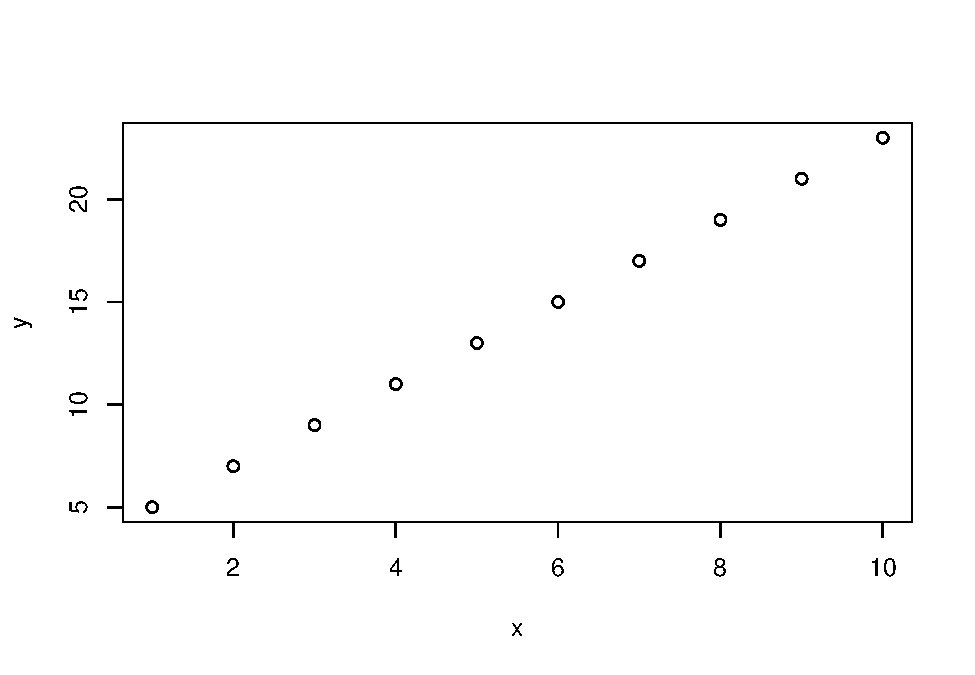
\includegraphics{test_course_notes_files/figure-latex/unnamed-chunk-4-1.pdf}

\hypertarget{getting-your-r-environment-set-up}{%
\section{Getting your R environment set up}\label{getting-your-r-environment-set-up}}

One of the first things you will have in any script or .rmd file is a section to load all the libraries that you use in that script.

You can install a library by using the install.packages() function, for example:

\texttt{install.packages("tidyverse")}, \texttt{install.packages("janitor")}, and \texttt{install.packages("psych")}

with this installed, you can then load the package using the library() function

\begin{Shaded}
\begin{Highlighting}[]
\KeywordTok{library}\NormalTok{(tidyverse)}
\end{Highlighting}
\end{Shaded}

\begin{verbatim}
## -- Attaching packages ------------ tidyverse 1.3.0 --
\end{verbatim}

\begin{verbatim}
## v ggplot2 3.3.2     v purrr   0.3.4
## v tibble  3.0.3     v dplyr   1.0.0
## v tidyr   1.1.0     v stringr 1.4.0
## v readr   1.3.1     v forcats 0.5.0
\end{verbatim}

\begin{verbatim}
## -- Conflicts --------------- tidyverse_conflicts() --
## x dplyr::filter() masks stats::filter()
## x dplyr::lag()    masks stats::lag()
\end{verbatim}

\begin{Shaded}
\begin{Highlighting}[]
\KeywordTok{library}\NormalTok{(janitor)}
\end{Highlighting}
\end{Shaded}

\begin{verbatim}
## Warning: package 'janitor' was built under R version 4.0.3
\end{verbatim}

\begin{verbatim}
## 
## Attaching package: 'janitor'
\end{verbatim}

\begin{verbatim}
## The following objects are masked from 'package:stats':
## 
##     chisq.test, fisher.test
\end{verbatim}

\begin{Shaded}
\begin{Highlighting}[]
\KeywordTok{library}\NormalTok{(psych)}
\end{Highlighting}
\end{Shaded}

\begin{verbatim}
## 
## Attaching package: 'psych'
\end{verbatim}

\begin{verbatim}
## The following objects are masked from 'package:ggplot2':
## 
##     %+%, alpha
\end{verbatim}

\hypertarget{reading-in-data}{%
\section{Reading in data}\label{reading-in-data}}

A good first step is to check which directory you are working in with the getwd() function

\texttt{getwd()}

You can also check which files are in that directory with \texttt{list.files()}.

If you notice that the file you are looking for is not there, then you can use setwd() to change your working directory

\texttt{setwd("./Week\ 2/")}

After that, make sure you have switched to the correct working directory
\texttt{getwd()} and then \texttt{list.files()}

Assuming you have directed yourself to the correct place, you can now read in the file(s) that you want to be working with.

\begin{Shaded}
\begin{Highlighting}[]
\NormalTok{prior\_survey \textless{}{-}}\StringTok{ }\KeywordTok{read\_csv}\NormalTok{(}\StringTok{"ENGE\_5714\_2021\_pre\_survey.csv"}\NormalTok{)}
\end{Highlighting}
\end{Shaded}

\begin{verbatim}
## Parsed with column specification:
## cols(
##   .default = col_character(),
##   student_id = col_double()
## )
\end{verbatim}

\begin{verbatim}
## See spec(...) for full column specifications.
\end{verbatim}

\hypertarget{exploring-the-data}{%
\section{Exploring the data}\label{exploring-the-data}}

Take a look at the csv

\begin{Shaded}
\begin{Highlighting}[]
\NormalTok{prior\_survey}
\end{Highlighting}
\end{Shaded}

\begin{verbatim}
## # A tibble: 24 x 49
##    student_id `I have taken a~ `I am intereste~ `I know what a ~
##         <dbl> <chr>            <chr>            <chr>           
##  1          1 Somewhat disagr~ Somewhat agree   Strongly disagr~
##  2          2 Strongly disagr~ Neither agree n~ Somewhat agree  
##  3          3 Strongly disagr~ Somewhat agree   Somewhat agree  
##  4          4 Somewhat disagr~ Strongly agree   Strongly disagr~
##  5          5 Somewhat agree   Strongly agree   Somewhat agree  
##  6          6 Somewhat disagr~ Somewhat agree   Somewhat disagr~
##  7          7 Strongly disagr~ Somewhat agree   Strongly disagr~
##  8          8 Somewhat agree   Somewhat agree   Somewhat agree  
##  9          9 Strongly disagr~ Strongly agree   Somewhat agree  
## 10         10 Neither agree n~ Strongly agree   Somewhat agree  
## # ... with 14 more rows, and 45 more variables: `I know what a type II error
## #   is` <chr>, `I know what a (statistical) confidence level is` <chr>, `I know
## #   what a p value is` <chr>, `I know what p-hacking means` <chr>, `I know what
## #   statistical power means` <chr>, `I have heard of frequentist statistics
## #   before` <chr>, `I have heard of Bayesian statistics before` <chr>, `I have
## #   heard the term "parametric statistics" before` <chr>, `I have heard the
## #   term "non-parametric statistics" before` <chr>, `I know what a histogram
## #   is.` <chr>, `I know what a probability distribution is.` <chr>, `I know
## #   what a random variable is.` <chr>, `I know what a probability distribution
## #   function is.` <chr>, `I know what a cumulative distribution function
## #   is.` <chr>, `I know what the expectation of a random variable is.` <chr>,
## #   `I know how to calculate the variance of a random variable.` <chr>, `I know
## #   what a z score is.` <chr>, `I know how to calculate the correlation between
## #   two variables.` <chr>, `I know how to interpret the correlation coefficient
## #   between two variables` <chr>, `I have heard of linear regression` <chr>, `I
## #   know how to run a linear regression (in some software...or by hand, if I'm
## #   feeling wild).` <chr>, `I know how to interpret a linear
## #   regression.` <chr>, `I have heard of multiple regression` <chr>, `I know
## #   how to perform a multiple regression` <chr>, `I know how to interpret a
## #   multiple regression` <chr>, `I have heard of logistic regression.` <chr>,
## #   `I understand when to use a logistic regression.` <chr>, `I know how to
## #   interpret the results of a logistic regression` <chr>, `I have heard of
## #   t-tests` <chr>, `I have performed a t-test before` <chr>, `I know how to
## #   interpret the results of a t-test` <chr>, `I have heard of Analysis of
## #   Variance.` <chr>, `I understand when to run an Analysis of Variance
## #   (ANOVA)` <chr>, `I know how to interpret the results from an ANOVA` <chr>,
## #   `I have heard of a chi-square test` <chr>, `I have used a chi-square test
## #   before` <chr>, `I know how to interpret the results of a chi-square
## #   test` <chr>, `I have heard of cluster analysis before` <chr>, `I have used
## #   cluster analysis before` <chr>, `I know how to interpret the results of a
## #   cluster analysis` <chr>, `I have heard of factor analysis (either
## #   exploratory or confirmatory)` <chr>, `I have used factor analysis (either
## #   exploratory or confirmatory)` <chr>, `I know how to interpret the results
## #   of a factor analysis (either exploratory or confirmatory)` <chr>, `I
## #   already have R and Rstudio downloaded to my computer.` <chr>, `I have used
## #   R before` <chr>
\end{verbatim}

Next, try cleaning the column names with \texttt{clean\_names()} from the janitor package.

\begin{Shaded}
\begin{Highlighting}[]
\NormalTok{prior\_survey \textless{}{-}}\StringTok{ }\NormalTok{prior\_survey }\OperatorTok{\%\textgreater{}\%}\StringTok{ }\KeywordTok{clean\_names}\NormalTok{() }\CommentTok{\# from janitor package}

\NormalTok{prior\_survey}\OperatorTok{$}\StringTok{\textasciigrave{}}\DataTypeTok{I have heard the term "non{-}parametric statistics" before}\StringTok{\textasciigrave{}}
\end{Highlighting}
\end{Shaded}

\begin{verbatim}
## Warning: Unknown or uninitialised column: `I have heard the term "non-parametric
## statistics" before`.
\end{verbatim}

\begin{verbatim}
## NULL
\end{verbatim}

\begin{Shaded}
\begin{Highlighting}[]
\KeywordTok{table}\NormalTok{(prior\_survey}\OperatorTok{$}\NormalTok{i\_have\_taken\_a\_quantitative\_research\_methods\_course\_before)}
\end{Highlighting}
\end{Shaded}

\begin{verbatim}
## 
## Neither agree nor disagree             Somewhat agree 
##                          2                          5 
##          Somewhat disagree             Strongly agree 
##                          5                          2 
##          Strongly disagree 
##                         10
\end{verbatim}

\hypertarget{plotting-data}{%
\section{Plotting data}\label{plotting-data}}

There are multiple ways to plot data. Focusing on using ggplot, here are two.

The first way passes the prior\_survey dataframe explicitly to ggplot

\begin{Shaded}
\begin{Highlighting}[]
\KeywordTok{ggplot}\NormalTok{(}\DataTypeTok{data =}\NormalTok{ prior\_survey, }\DataTypeTok{mapping =} \KeywordTok{aes}\NormalTok{(}\DataTypeTok{x =}\NormalTok{ i\_know\_what\_a\_type\_i\_error\_is)) }\OperatorTok{+}
\StringTok{  }\KeywordTok{geom\_bar}\NormalTok{() }\OperatorTok{+}
\StringTok{  }\KeywordTok{coord\_flip}\NormalTok{()}
\end{Highlighting}
\end{Shaded}

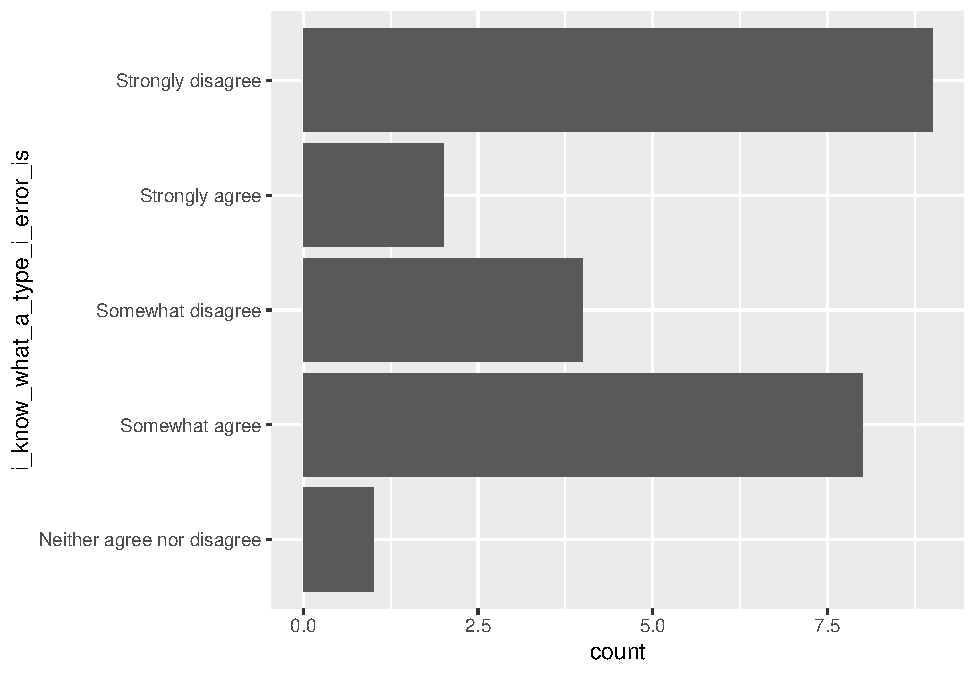
\includegraphics{test_course_notes_files/figure-latex/unnamed-chunk-9-1.pdf}

The second way does this implicitly, using the pipe operator. Note that the results should be the same.

\begin{Shaded}
\begin{Highlighting}[]
\NormalTok{prior\_survey }\OperatorTok{\%\textgreater{}\%}\StringTok{ }
\StringTok{  }\KeywordTok{ggplot}\NormalTok{(}\DataTypeTok{mapping =} \KeywordTok{aes}\NormalTok{(}\DataTypeTok{x =}\NormalTok{ i\_know\_what\_a\_type\_i\_error\_is)) }\OperatorTok{+}
\StringTok{  }\KeywordTok{geom\_bar}\NormalTok{() }\OperatorTok{+}
\StringTok{  }\KeywordTok{coord\_flip}\NormalTok{()}
\end{Highlighting}
\end{Shaded}

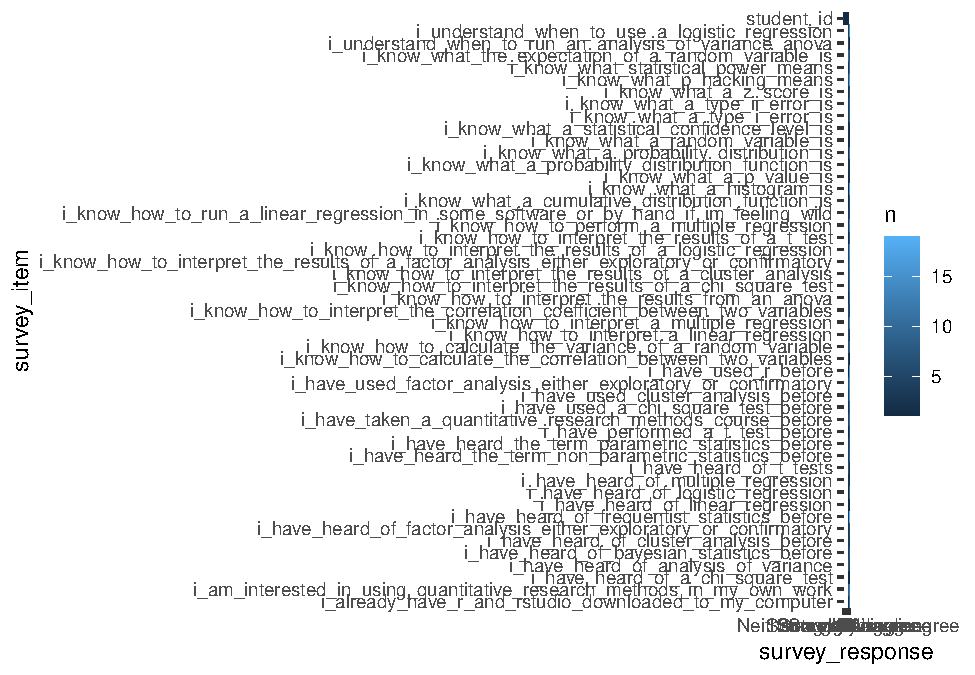
\includegraphics{test_course_notes_files/figure-latex/unnamed-chunk-10-1.pdf}

If we wanted to get extra fancy, we could first convert the data from a wide format to a long format and then start plotting all the items together.

Converting to long format would produce something like this:

\begin{Shaded}
\begin{Highlighting}[]
\NormalTok{prior\_survey }\OperatorTok{\%\textgreater{}\%}\StringTok{ }
\StringTok{  }\KeywordTok{gather}\NormalTok{(}\DataTypeTok{key =} \StringTok{"survey\_item"}\NormalTok{, }\DataTypeTok{value =} \StringTok{"survey\_response"}\NormalTok{)}
\end{Highlighting}
\end{Shaded}

\begin{verbatim}
## # A tibble: 1,176 x 2
##    survey_item survey_response
##    <chr>       <chr>          
##  1 student_id  1              
##  2 student_id  2              
##  3 student_id  3              
##  4 student_id  4              
##  5 student_id  5              
##  6 student_id  6              
##  7 student_id  7              
##  8 student_id  8              
##  9 student_id  9              
## 10 student_id  10             
## # ... with 1,166 more rows
\end{verbatim}

Then we can combine that with the \texttt{group\_by()} and \texttt{summarize()} functions and plot the results.

\begin{Shaded}
\begin{Highlighting}[]
\NormalTok{prior\_survey }\OperatorTok{\%\textgreater{}\%}\StringTok{ }
\StringTok{  }\KeywordTok{gather}\NormalTok{(}\DataTypeTok{key =} \StringTok{"survey\_item"}\NormalTok{, }\DataTypeTok{value =} \StringTok{"survey\_response"}\NormalTok{) }\OperatorTok{\%\textgreater{}\%}\StringTok{ }
\StringTok{  }\KeywordTok{group\_by}\NormalTok{(survey\_item, survey\_response) }\OperatorTok{\%\textgreater{}\%}\StringTok{ }
\StringTok{  }\KeywordTok{summarize}\NormalTok{(}\DataTypeTok{n =} \KeywordTok{n}\NormalTok{()) }\OperatorTok{\%\textgreater{}\%}\StringTok{ }
\StringTok{  }\KeywordTok{ggplot}\NormalTok{(}\DataTypeTok{mapping =} \KeywordTok{aes}\NormalTok{(}\DataTypeTok{x =}\NormalTok{ survey\_response, }\DataTypeTok{y =}\NormalTok{ survey\_item, }\DataTypeTok{fill =}\NormalTok{ n)) }\OperatorTok{+}
\StringTok{  }\KeywordTok{geom\_tile}\NormalTok{()}
\end{Highlighting}
\end{Shaded}

\begin{verbatim}
## `summarise()` regrouping output by 'survey_item' (override with `.groups` argument)
\end{verbatim}

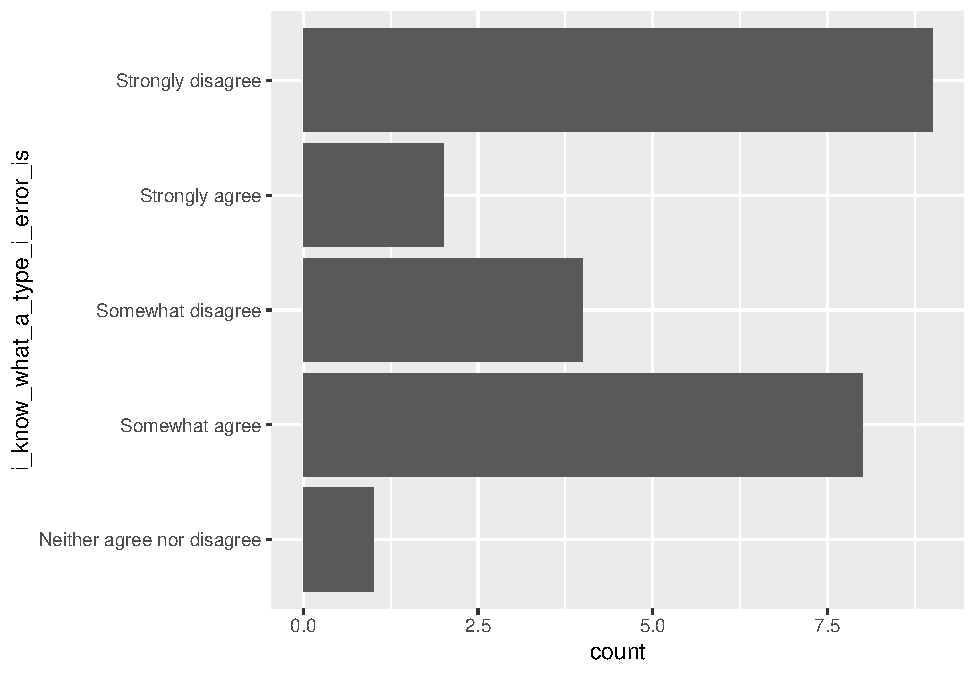
\includegraphics{test_course_notes_files/figure-latex/unnamed-chunk-12-1.pdf}

This plot is okay for giving a general sense of what is going on in these plots but there are a bunch of other ways to go about doing this.

First, maybe we want to rename the response categories to a numerical scale. We can accomplish this with a \texttt{mutate()} and \texttt{case\_when()}.

\begin{Shaded}
\begin{Highlighting}[]
\NormalTok{prior\_survey \textless{}{-}}\StringTok{ }\NormalTok{prior\_survey }\OperatorTok{\%\textgreater{}\%}\StringTok{ }
\StringTok{  }\KeywordTok{gather}\NormalTok{(}\DataTypeTok{key =} \StringTok{"survey\_item"}\NormalTok{, }\DataTypeTok{value =} \StringTok{"survey\_response"}\NormalTok{) }\OperatorTok{\%\textgreater{}\%}\StringTok{ }
\StringTok{  }\KeywordTok{mutate}\NormalTok{(}\DataTypeTok{survey\_response\_num =} \KeywordTok{case\_when}\NormalTok{(survey\_response }\OperatorTok{==}\StringTok{ "Strongly disagree"} \OperatorTok{\textasciitilde{}}\StringTok{ }\DecValTok{0}\NormalTok{,}
\NormalTok{                                         survey\_response }\OperatorTok{==}\StringTok{ "Somewhat disagree"} \OperatorTok{\textasciitilde{}}\StringTok{ }\DecValTok{1}\NormalTok{,}
\NormalTok{                                         survey\_response }\OperatorTok{==}\StringTok{ "Neither agree nor disagree"} \OperatorTok{\textasciitilde{}}\StringTok{ }\DecValTok{2}\NormalTok{,}
\NormalTok{                                         survey\_response }\OperatorTok{==}\StringTok{ "Somewhat agree"} \OperatorTok{\textasciitilde{}}\StringTok{ }\DecValTok{3}\NormalTok{,}
\NormalTok{                                         survey\_response }\OperatorTok{==}\StringTok{ "Strongly agree"} \OperatorTok{\textasciitilde{}}\StringTok{ }\DecValTok{4}\NormalTok{,}
\NormalTok{                                         )) }
\end{Highlighting}
\end{Shaded}

Then we plot the same data but with the numerical scale along the x-axis.

\begin{Shaded}
\begin{Highlighting}[]
\NormalTok{prior\_survey }\OperatorTok{\%\textgreater{}\%}\StringTok{ }
\StringTok{  }\KeywordTok{group\_by}\NormalTok{(survey\_item, survey\_response\_num) }\OperatorTok{\%\textgreater{}\%}\StringTok{ }
\StringTok{  }\KeywordTok{summarize}\NormalTok{(}\DataTypeTok{n =} \KeywordTok{n}\NormalTok{()) }\OperatorTok{\%\textgreater{}\%}\StringTok{ }
\StringTok{  }\KeywordTok{ggplot}\NormalTok{(}\DataTypeTok{mapping =} \KeywordTok{aes}\NormalTok{(}\DataTypeTok{x =}\NormalTok{ survey\_response\_num, }\DataTypeTok{y =}\NormalTok{ survey\_item, }\DataTypeTok{fill =}\NormalTok{ n)) }\OperatorTok{+}
\StringTok{  }\KeywordTok{geom\_tile}\NormalTok{()}
\end{Highlighting}
\end{Shaded}

\begin{verbatim}
## `summarise()` regrouping output by 'survey_item' (override with `.groups` argument)
\end{verbatim}

\begin{verbatim}
## Warning: Removed 3 rows containing missing values (geom_tile).
\end{verbatim}

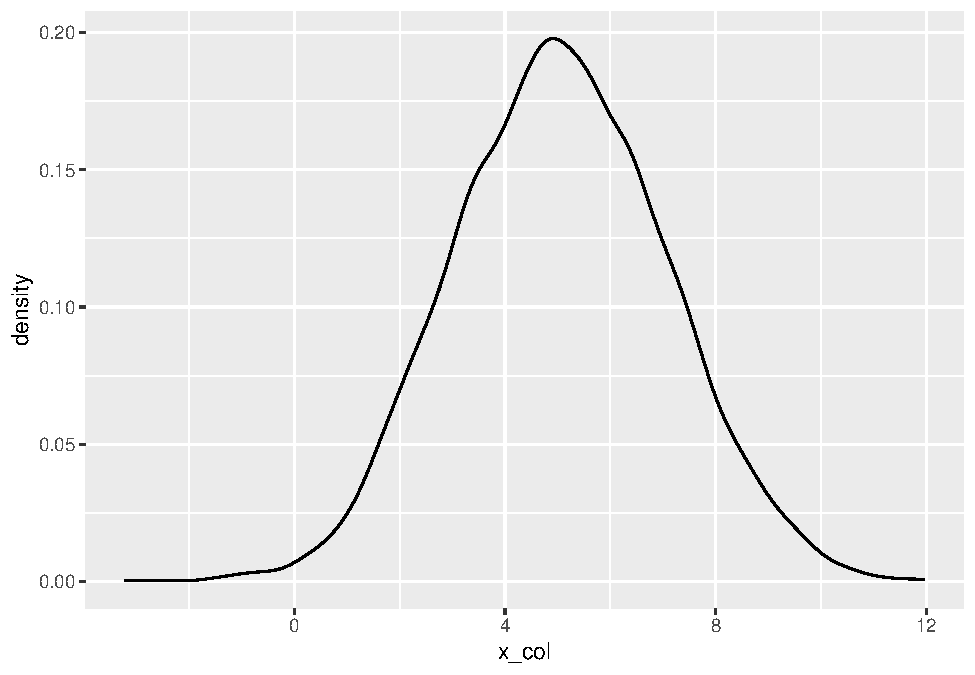
\includegraphics{test_course_notes_files/figure-latex/unnamed-chunk-14-1.pdf}

\hypertarget{week-3---data-cleaning-organizing-describing-and-communicating}{%
\chapter{Week 3 - Data Cleaning, Organizing, Describing, and Communicating}\label{week-3---data-cleaning-organizing-describing-and-communicating}}

\hypertarget{one-continuous-variable-either-predictor-or-outcome-variable}{%
\section{One continuous variable (either predictor or outcome variable)}\label{one-continuous-variable-either-predictor-or-outcome-variable}}

\begin{Shaded}
\begin{Highlighting}[]
\NormalTok{num \textless{}{-}}\StringTok{ }\DecValTok{50}
\NormalTok{mu \textless{}{-}}\StringTok{ }\DecValTok{5}
\NormalTok{stdev \textless{}{-}}\StringTok{ }\DecValTok{2}

\NormalTok{x \textless{}{-}}\StringTok{ }\KeywordTok{rnorm}\NormalTok{(}\DataTypeTok{n =}\NormalTok{ num, }\DataTypeTok{mean =}\NormalTok{ mu, }\DataTypeTok{sd =}\NormalTok{ stdev)}
\KeywordTok{hist}\NormalTok{(x)}
\end{Highlighting}
\end{Shaded}

You can also do this using ggplot rather than base R graphics

\begin{Shaded}
\begin{Highlighting}[]
\NormalTok{num \textless{}{-}}\StringTok{ }\DecValTok{50}
\NormalTok{mu \textless{}{-}}\StringTok{ }\DecValTok{5}
\NormalTok{stdev \textless{}{-}}\StringTok{ }\DecValTok{2}

\NormalTok{x\_vec \textless{}{-}}\StringTok{ }\KeywordTok{rnorm}\NormalTok{(}\DataTypeTok{n =}\NormalTok{ num, }\DataTypeTok{mean =}\NormalTok{ mu, }\DataTypeTok{sd =}\NormalTok{ stdev)}
\NormalTok{x\_df \textless{}{-}}\StringTok{ }\KeywordTok{tibble}\NormalTok{(}\DataTypeTok{x\_col =}\NormalTok{ x\_vec)}

\KeywordTok{ggplot}\NormalTok{(}\DataTypeTok{data =}\NormalTok{ x\_df, }\DataTypeTok{mapping =} \KeywordTok{aes}\NormalTok{(}\DataTypeTok{x =}\NormalTok{ x)) }\OperatorTok{+}
\StringTok{  }\KeywordTok{geom\_histogram}\NormalTok{()}
\end{Highlighting}
\end{Shaded}

\begin{verbatim}
## `stat_bin()` using `bins = 30`. Pick better value with `binwidth`.
\end{verbatim}

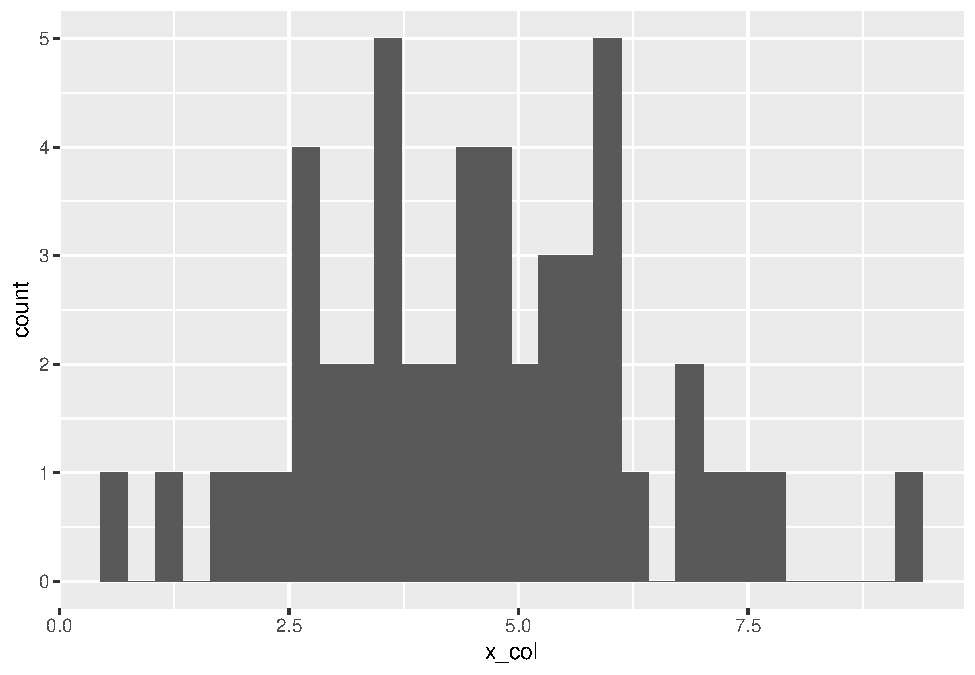
\includegraphics{test_course_notes_files/figure-latex/ggplot-hist-1.pdf}

You can use geom\_density() instead of geom\_histogram() to get a smooth graph

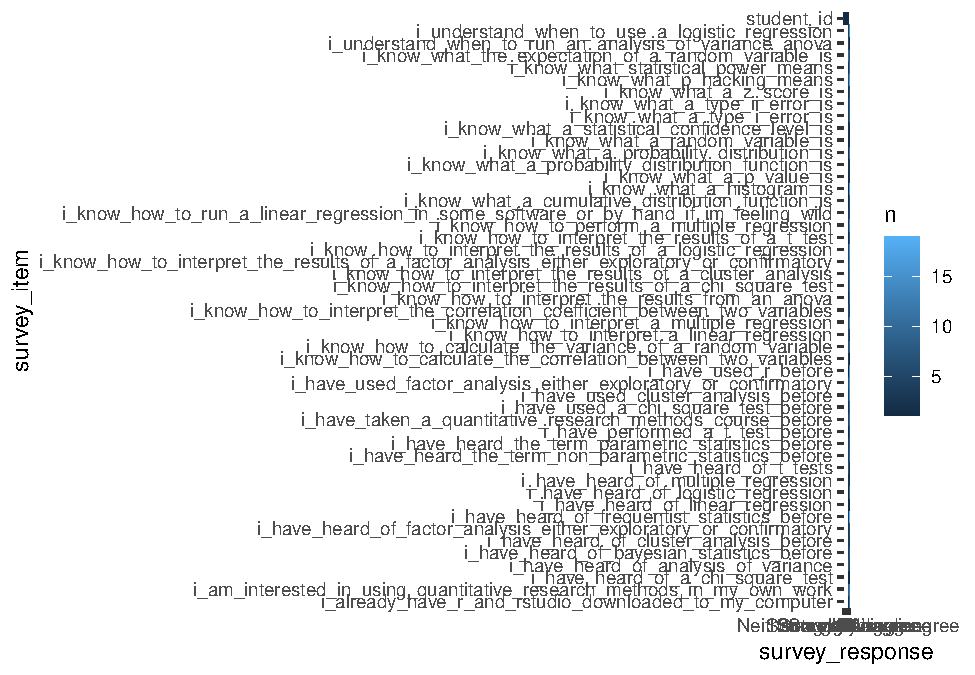
\includegraphics{test_course_notes_files/figure-latex/unnamed-chunk-15-1.pdf} 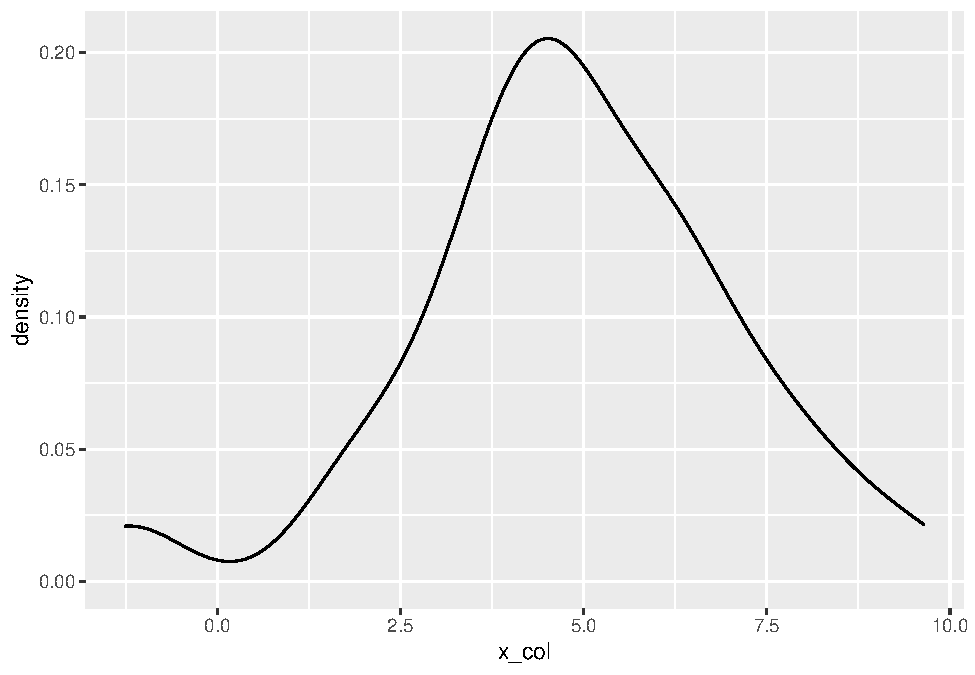
\includegraphics{test_course_notes_files/figure-latex/unnamed-chunk-15-2.pdf} 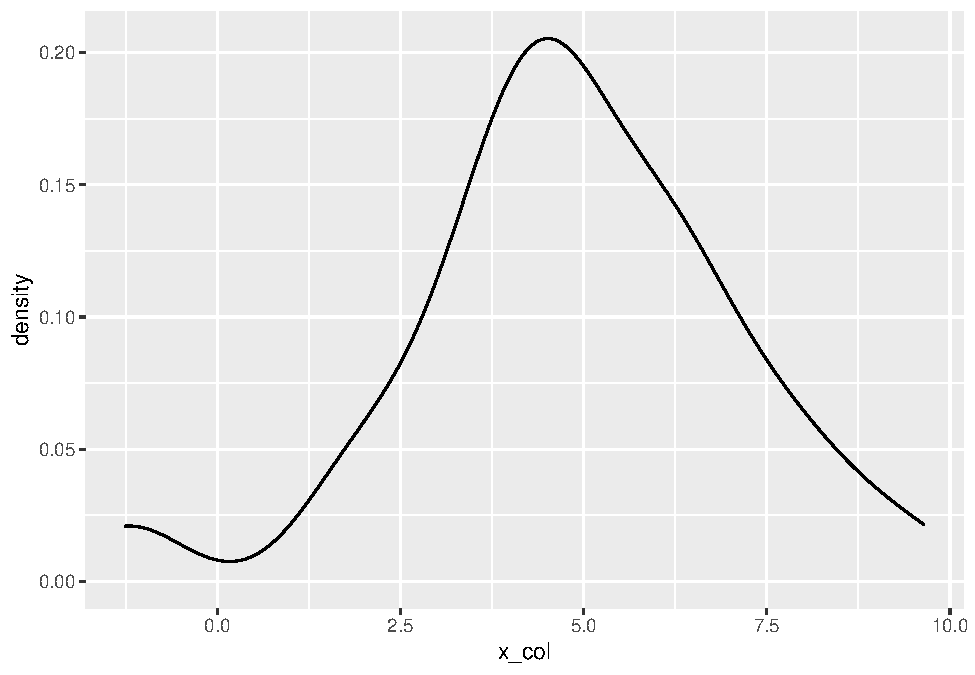
\includegraphics{test_course_notes_files/figure-latex/unnamed-chunk-15-3.pdf}

Just for fun, look at what happens to the the plot if you increase the sample size

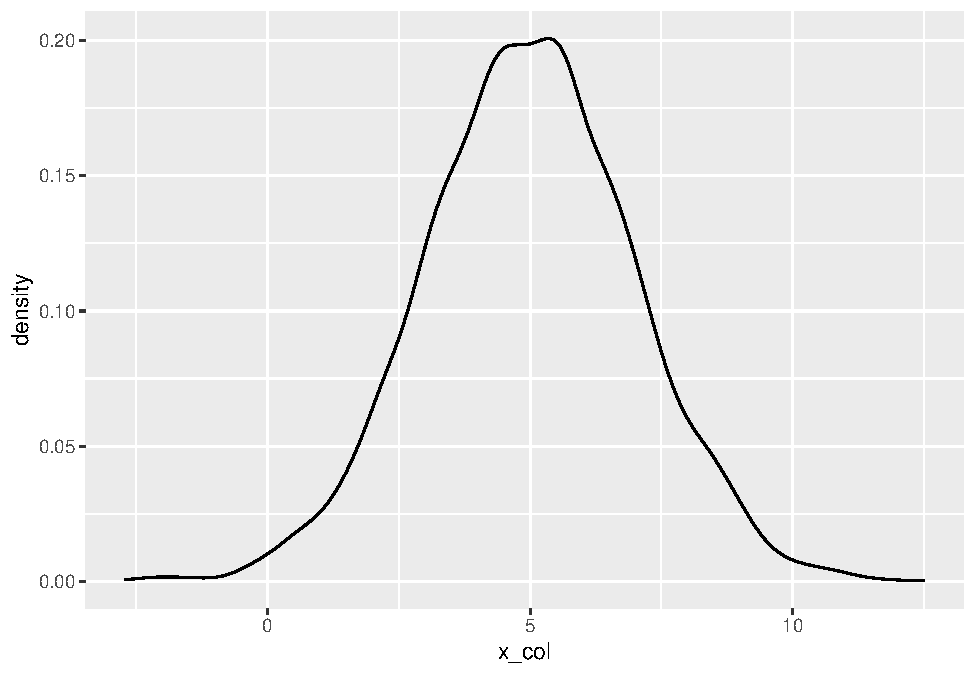
\includegraphics{test_course_notes_files/figure-latex/unnamed-chunk-16-1.pdf}

\hypertarget{one-discrete-variable-either-predictor-or-outcome}{%
\section{One Discrete Variable (either predictor or outcome)}\label{one-discrete-variable-either-predictor-or-outcome}}

\begin{Shaded}
\begin{Highlighting}[]
\CommentTok{\#\# load in the data}
\NormalTok{survey\_df \textless{}{-}}\StringTok{ }\KeywordTok{read\_csv}\NormalTok{(}\StringTok{"ENGE\_5714\_2021\_pre\_survey.csv"}\NormalTok{)}
\end{Highlighting}
\end{Shaded}

\begin{verbatim}
## Parsed with column specification:
## cols(
##   .default = col_character(),
##   student_id = col_double()
## )
\end{verbatim}

\begin{verbatim}
## See spec(...) for full column specifications.
\end{verbatim}

\begin{Shaded}
\begin{Highlighting}[]
\NormalTok{survey\_df \textless{}{-}}\StringTok{ }\NormalTok{survey\_df }\OperatorTok{\%\textgreater{}\%}\StringTok{ }\KeywordTok{clean\_names}\NormalTok{()}
\end{Highlighting}
\end{Shaded}

\begin{Shaded}
\begin{Highlighting}[]
\NormalTok{survey\_df }\OperatorTok{\%\textgreater{}\%}\StringTok{ }
\StringTok{  }\KeywordTok{ggplot}\NormalTok{(}\KeywordTok{aes}\NormalTok{(}\DataTypeTok{x =}\NormalTok{ i\_have\_taken\_a\_quantitative\_research\_methods\_course\_before)) }\OperatorTok{+}
\StringTok{  }\KeywordTok{geom\_bar}\NormalTok{()}
\end{Highlighting}
\end{Shaded}

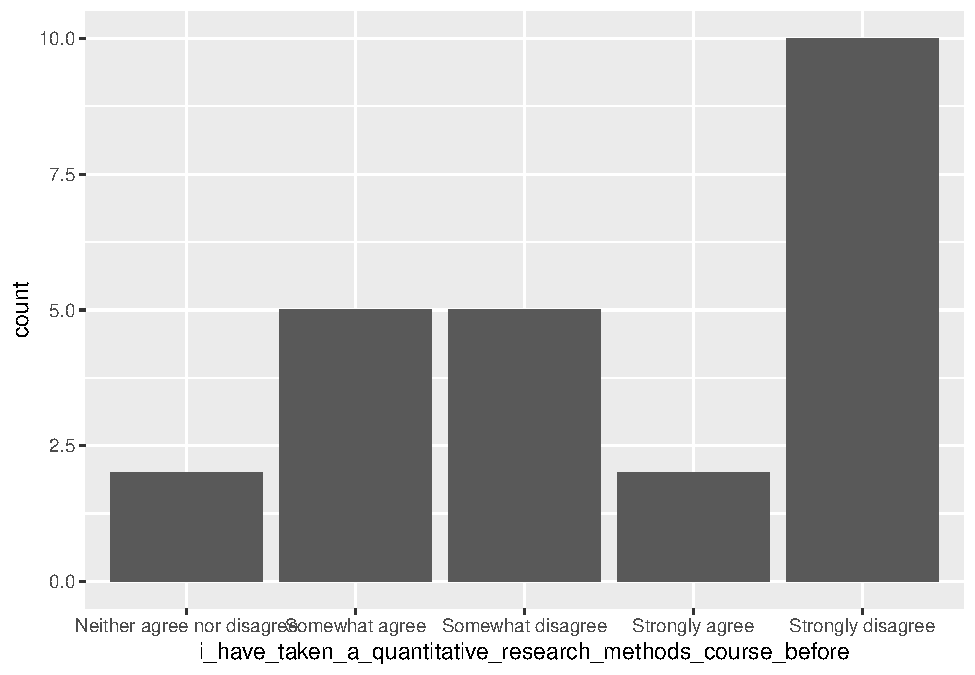
\includegraphics{test_course_notes_files/figure-latex/geom-bar-1.pdf}

Notice that the ordering is not quite what we would want. It is alphabetical. Try to find how we can fix this.

Here is one way:

\begin{Shaded}
\begin{Highlighting}[]
\NormalTok{q\_levels \textless{}{-}}\StringTok{ }\KeywordTok{c}\NormalTok{(}\StringTok{"Strongly disagree"}\NormalTok{, }\StringTok{"Somewhat disagree"}\NormalTok{, }\StringTok{"Neither agree nor disagree"}\NormalTok{,}
              \StringTok{"Somewhat agree"}\NormalTok{, }\StringTok{"Strongly agree"}\NormalTok{)}



\NormalTok{survey\_df}\OperatorTok{$}\NormalTok{i\_have\_taken\_a\_quantitative\_research\_methods\_course\_before \textless{}{-}}\StringTok{ }\KeywordTok{factor}\NormalTok{(survey\_df}\OperatorTok{$}\NormalTok{i\_have\_taken\_a\_quantitative\_research\_methods\_course\_before, }
                                                                               \DataTypeTok{levels =}\NormalTok{ q\_levels,}
                                                                               \DataTypeTok{ordered =} \OtherTok{TRUE}\NormalTok{)}


\CommentTok{\#\# Now try plotting}

\NormalTok{survey\_df }\OperatorTok{\%\textgreater{}\%}\StringTok{ }
\StringTok{  }\KeywordTok{ggplot}\NormalTok{(}\KeywordTok{aes}\NormalTok{(}\DataTypeTok{x =}\NormalTok{ i\_have\_taken\_a\_quantitative\_research\_methods\_course\_before)) }\OperatorTok{+}
\StringTok{  }\KeywordTok{geom\_bar}\NormalTok{() }\OperatorTok{+}
\StringTok{  }\KeywordTok{coord\_flip}\NormalTok{() }\OperatorTok{+}
\StringTok{  }\KeywordTok{labs}\NormalTok{(}\DataTypeTok{x =} \StringTok{"I have taken a quantitative research methods course before"}\NormalTok{,}
       \DataTypeTok{y =} \StringTok{"Count"}\NormalTok{,}
       \DataTypeTok{title =} \StringTok{"Reordered Example"}\NormalTok{)}
\end{Highlighting}
\end{Shaded}

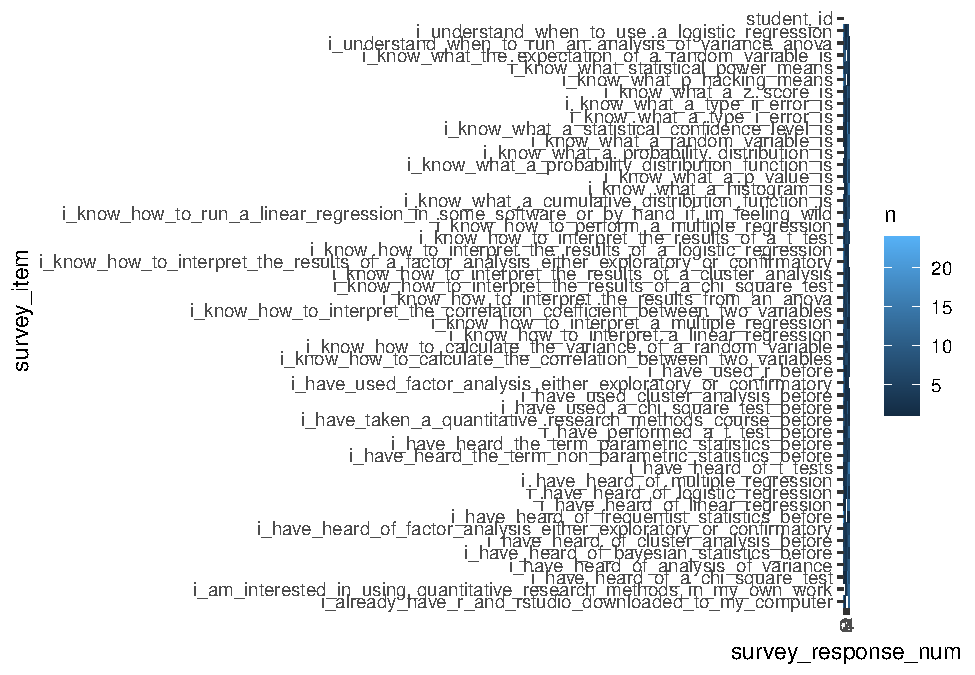
\includegraphics{test_course_notes_files/figure-latex/unnamed-chunk-17-1.pdf}

\hypertarget{joining-two-datasets}{%
\subsection{Joining two datasets}\label{joining-two-datasets}}

Let's imagine that we have a separate dataset that has information about the students who completed the pre-course prior knowledge survey.

First, we will load in that dataset

\begin{Shaded}
\begin{Highlighting}[]
\NormalTok{survey\_info\_df \textless{}{-}}\StringTok{ }\KeywordTok{read\_csv}\NormalTok{(}\StringTok{"survey\_student\_info.csv"}\NormalTok{)}
\end{Highlighting}
\end{Shaded}

\begin{verbatim}
## Parsed with column specification:
## cols(
##   student_id = col_double(),
##   standing = col_character(),
##   college = col_character(),
##   required = col_character()
## )
\end{verbatim}

Next, let's join the two datasets based on the student id column, which is in each of the two dataframes.

\begin{Shaded}
\begin{Highlighting}[]
\NormalTok{survey\_df \textless{}{-}}\StringTok{ }\NormalTok{survey\_df }\OperatorTok{\%\textgreater{}\%}\StringTok{ }\KeywordTok{inner\_join}\NormalTok{(survey\_info\_df, }\DataTypeTok{by =} \StringTok{"student\_id"}\NormalTok{)}
\end{Highlighting}
\end{Shaded}

Now we should have both datasets joined into one and saved as survey\_df.

With this, we can make some nicer plots and do something like use facet\_grid() to look at students who are masters and doctoral students, for example.

\begin{Shaded}
\begin{Highlighting}[]
\NormalTok{survey\_df }\OperatorTok{\%\textgreater{}\%}\StringTok{ }
\StringTok{  }\KeywordTok{ggplot}\NormalTok{(}\KeywordTok{aes}\NormalTok{(}\DataTypeTok{x =}\NormalTok{ i\_have\_taken\_a\_quantitative\_research\_methods\_course\_before)) }\OperatorTok{+}
\StringTok{  }\KeywordTok{geom\_bar}\NormalTok{() }\OperatorTok{+}
\StringTok{  }\KeywordTok{facet\_grid}\NormalTok{(standing }\OperatorTok{\textasciitilde{}}\NormalTok{.) }\OperatorTok{+}
\StringTok{  }\KeywordTok{labs}\NormalTok{(}\DataTypeTok{x =} \StringTok{"I have taken a quantitative research methods course before"}\NormalTok{,}
       \DataTypeTok{y =} \StringTok{"Count"}\NormalTok{,}
       \DataTypeTok{title =} \StringTok{"Reordered Example"}\NormalTok{)}
\end{Highlighting}
\end{Shaded}

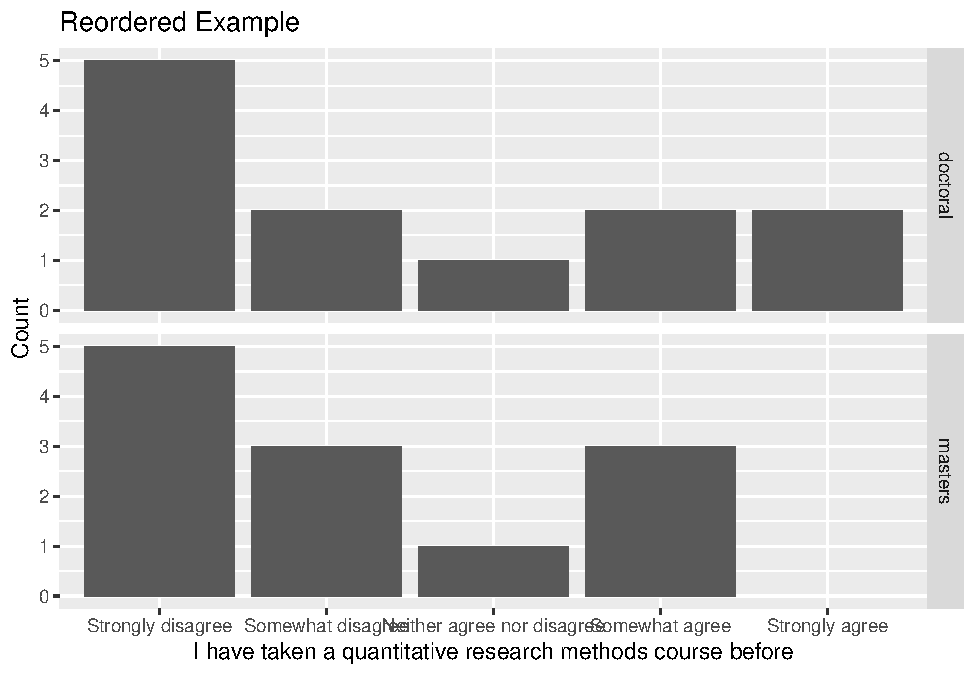
\includegraphics{test_course_notes_files/figure-latex/unnamed-chunk-20-1.pdf}

The x axis looks a little crowded. What if we try coord\_flip()

\begin{Shaded}
\begin{Highlighting}[]
\NormalTok{survey\_df }\OperatorTok{\%\textgreater{}\%}\StringTok{ }
\StringTok{  }\KeywordTok{filter}\NormalTok{(standing }\OperatorTok{==}\StringTok{ "doctoral"}\NormalTok{) }\OperatorTok{\%\textgreater{}\%}
\StringTok{  }\KeywordTok{ggplot}\NormalTok{(}\KeywordTok{aes}\NormalTok{(}\DataTypeTok{x =}\NormalTok{ i\_have\_taken\_a\_quantitative\_research\_methods\_course\_before)) }\OperatorTok{+}
\StringTok{  }\KeywordTok{geom\_bar}\NormalTok{() }\OperatorTok{+}
\StringTok{  }\KeywordTok{coord\_flip}\NormalTok{() }\OperatorTok{+}
\StringTok{  }\KeywordTok{facet\_grid}\NormalTok{(standing }\OperatorTok{\textasciitilde{}}\NormalTok{.) }\OperatorTok{+}
\StringTok{  }\KeywordTok{labs}\NormalTok{(}\DataTypeTok{x =} \StringTok{"I have taken a quantitative research methods course before"}\NormalTok{,}
       \DataTypeTok{y =} \StringTok{"Count"}\NormalTok{,}
       \DataTypeTok{title =} \StringTok{"Reordered Example"}\NormalTok{)}
\end{Highlighting}
\end{Shaded}

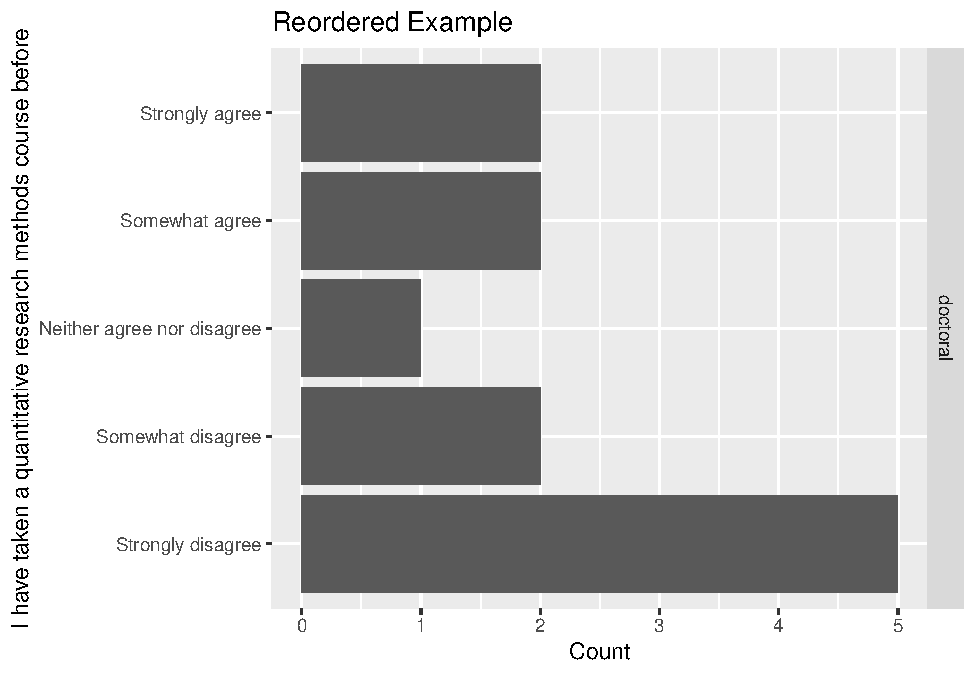
\includegraphics{test_course_notes_files/figure-latex/unnamed-chunk-21-1.pdf}

A quick note on filters

\begin{Shaded}
\begin{Highlighting}[]
\NormalTok{survey\_df }\OperatorTok{\%\textgreater{}\%}\StringTok{ }\KeywordTok{filter}\NormalTok{(required }\OperatorTok{==}\StringTok{ "yes"}\NormalTok{)}
\end{Highlighting}
\end{Shaded}

\begin{verbatim}
## # A tibble: 12 x 52
##    student_id i_have_taken_a_~ i_am_interested~ i_know_what_a_t~
##         <dbl> <ord>            <chr>            <chr>           
##  1          1 Somewhat disagr~ Somewhat agree   Strongly disagr~
##  2          2 Strongly disagr~ Neither agree n~ Somewhat agree  
##  3          4 Somewhat disagr~ Strongly agree   Strongly disagr~
##  4          8 Somewhat agree   Somewhat agree   Somewhat agree  
##  5          9 Strongly disagr~ Strongly agree   Somewhat agree  
##  6         11 Strongly disagr~ Strongly agree   Strongly disagr~
##  7         16 Strongly agree   Strongly agree   Somewhat agree  
##  8         17 Strongly disagr~ Strongly agree   Strongly disagr~
##  9         18 Somewhat disagr~ Somewhat agree   Somewhat disagr~
## 10         20 Strongly disagr~ Neither agree n~ Neither agree n~
## 11         22 Strongly disagr~ Strongly agree   Strongly disagr~
## 12         23 Somewhat agree   Strongly agree   Somewhat agree  
## # ... with 48 more variables: i_know_what_a_type_ii_error_is <chr>,
## #   i_know_what_a_statistical_confidence_level_is <chr>,
## #   i_know_what_a_p_value_is <chr>, i_know_what_p_hacking_means <chr>,
## #   i_know_what_statistical_power_means <chr>,
## #   i_have_heard_of_frequentist_statistics_before <chr>,
## #   i_have_heard_of_bayesian_statistics_before <chr>,
## #   i_have_heard_the_term_parametric_statistics_before <chr>,
## #   i_have_heard_the_term_non_parametric_statistics_before <chr>,
## #   i_know_what_a_histogram_is <chr>,
## #   i_know_what_a_probability_distribution_is <chr>,
## #   i_know_what_a_random_variable_is <chr>,
## #   i_know_what_a_probability_distribution_function_is <chr>,
## #   i_know_what_a_cumulative_distribution_function_is <chr>,
## #   i_know_what_the_expectation_of_a_random_variable_is <chr>,
## #   i_know_how_to_calculate_the_variance_of_a_random_variable <chr>,
## #   i_know_what_a_z_score_is <chr>,
## #   i_know_how_to_calculate_the_correlation_between_two_variables <chr>,
## #   i_know_how_to_interpret_the_correlation_coefficient_between_two_variables <chr>,
## #   i_have_heard_of_linear_regression <chr>,
## #   i_know_how_to_run_a_linear_regression_in_some_software_or_by_hand_if_im_feeling_wild <chr>,
## #   i_know_how_to_interpret_a_linear_regression <chr>,
## #   i_have_heard_of_multiple_regression <chr>,
## #   i_know_how_to_perform_a_multiple_regression <chr>,
## #   i_know_how_to_interpret_a_multiple_regression <chr>,
## #   i_have_heard_of_logistic_regression <chr>,
## #   i_understand_when_to_use_a_logistic_regression <chr>,
## #   i_know_how_to_interpret_the_results_of_a_logistic_regression <chr>,
## #   i_have_heard_of_t_tests <chr>, i_have_performed_a_t_test_before <chr>,
## #   i_know_how_to_interpret_the_results_of_a_t_test <chr>,
## #   i_have_heard_of_analysis_of_variance <chr>,
## #   i_understand_when_to_run_an_analysis_of_variance_anova <chr>,
## #   i_know_how_to_interpret_the_results_from_an_anova <chr>,
## #   i_have_heard_of_a_chi_square_test <chr>,
## #   i_have_used_a_chi_square_test_before <chr>,
## #   i_know_how_to_interpret_the_results_of_a_chi_square_test <chr>,
## #   i_have_heard_of_cluster_analysis_before <chr>,
## #   i_have_used_cluster_analysis_before <chr>,
## #   i_know_how_to_interpret_the_results_of_a_cluster_analysis <chr>,
## #   i_have_heard_of_factor_analysis_either_exploratory_or_confirmatory <chr>,
## #   i_have_used_factor_analysis_either_exploratory_or_confirmatory <chr>,
## #   i_know_how_to_interpret_the_results_of_a_factor_analysis_either_exploratory_or_confirmatory <chr>,
## #   i_already_have_r_and_rstudio_downloaded_to_my_computer <chr>,
## #   i_have_used_r_before <chr>, standing <chr>, college <chr>, required <chr>
\end{verbatim}

\begin{Shaded}
\begin{Highlighting}[]
\NormalTok{filtered\_df \textless{}{-}}\StringTok{ }\NormalTok{survey\_df }\OperatorTok{\%\textgreater{}\%}\StringTok{ }\KeywordTok{filter}\NormalTok{(required }\OperatorTok{==}\StringTok{ "yes"}\NormalTok{)}
\end{Highlighting}
\end{Shaded}

\hypertarget{a-little-more-about-plotting}{%
\subsubsection{A little more about plotting}\label{a-little-more-about-plotting}}

We are going to shift gears again and look at a few different kinds of plots. The main thing to remember here is that you want to think about whether the variables you have are nominal, ordinal, or continuous (that includes interval and ratio).

\hypertarget{discrete-predictor-continuous-outcome}{%
\section{Discrete Predictor, Continuous Outcome}\label{discrete-predictor-continuous-outcome}}

\begin{Shaded}
\begin{Highlighting}[]
\NormalTok{group\_size \textless{}{-}}\StringTok{ }\DecValTok{20}
\NormalTok{chem\_e\_scores \textless{}{-}}\StringTok{ }\KeywordTok{rnorm}\NormalTok{(}\DataTypeTok{n =}\NormalTok{ group\_size, }\DataTypeTok{mean =} \DecValTok{85}\NormalTok{, }\DataTypeTok{sd =} \DecValTok{4}\NormalTok{)}
\NormalTok{chem\_scores \textless{}{-}}\StringTok{ }\KeywordTok{rnorm}\NormalTok{(}\DataTypeTok{n =}\NormalTok{ group\_size, }\DataTypeTok{mean =} \DecValTok{78}\NormalTok{, }\DataTypeTok{sd =} \DecValTok{6}\NormalTok{)}


\NormalTok{data\_df \textless{}{-}}\StringTok{ }\KeywordTok{tibble}\NormalTok{(}
  \DataTypeTok{discipline =} \KeywordTok{rep}\NormalTok{(}\KeywordTok{c}\NormalTok{(}\StringTok{"ChemE"}\NormalTok{, }\StringTok{"Chemistry"}\NormalTok{), }\DataTypeTok{each =}\NormalTok{ group\_size),}
  \DataTypeTok{score =} \KeywordTok{c}\NormalTok{(chem\_e\_scores, chem\_scores)}
\NormalTok{)}

\NormalTok{data\_df }\OperatorTok{\%\textgreater{}\%}\StringTok{ }
\StringTok{  }\KeywordTok{ggplot}\NormalTok{(}\KeywordTok{aes}\NormalTok{(}\DataTypeTok{x =}\NormalTok{ discipline, }\DataTypeTok{y =}\NormalTok{ score)) }\OperatorTok{+}
\StringTok{  }\KeywordTok{geom\_boxplot}\NormalTok{()}
\end{Highlighting}
\end{Shaded}

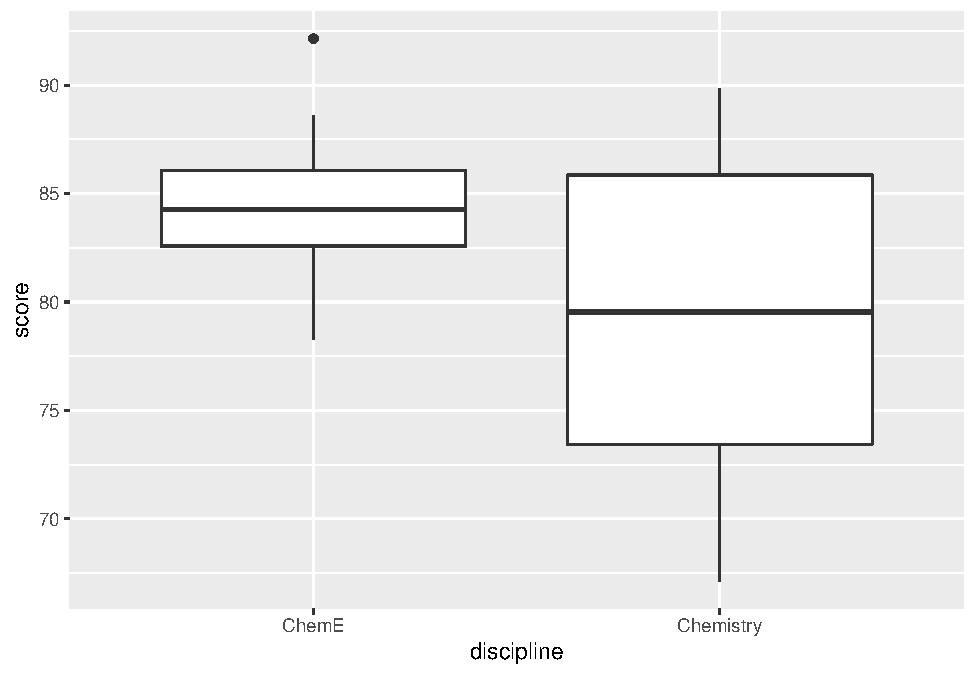
\includegraphics{test_course_notes_files/figure-latex/boxplot-example-1.pdf}

You can make a few modifications to possibly make this easier to read.

The first is to put the discrete category on the y axis instead of the x axis.

The second is to use geom\_jitter() in addition to geom\_boxplot() to show the individual points in each group.

\begin{Shaded}
\begin{Highlighting}[]
\NormalTok{data\_df }\OperatorTok{\%\textgreater{}\%}\StringTok{ }
\StringTok{  }\KeywordTok{ggplot}\NormalTok{(}\KeywordTok{aes}\NormalTok{(}\DataTypeTok{y =}\NormalTok{ score, }\DataTypeTok{x =}\NormalTok{ discipline)) }\OperatorTok{+}
\StringTok{  }\KeywordTok{geom\_boxplot}\NormalTok{() }\OperatorTok{+}
\StringTok{  }\KeywordTok{geom\_jitter}\NormalTok{()}
\end{Highlighting}
\end{Shaded}

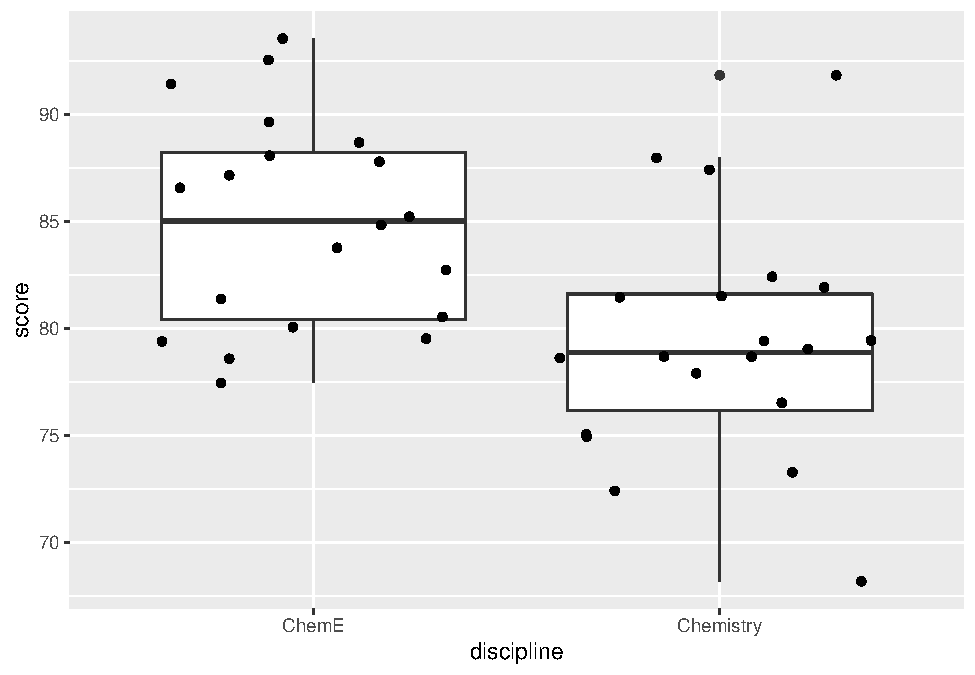
\includegraphics{test_course_notes_files/figure-latex/box-and-dot-plot-1.pdf}

\hypertarget{continuous-predictor-and-continuous-outcome}{%
\section{Continuous predictor and continuous outcome}\label{continuous-predictor-and-continuous-outcome}}

First, let's re-do a lot of the steps in this week's script for reading in data and transforming it a little

\begin{Shaded}
\begin{Highlighting}[]
\NormalTok{mydata \textless{}{-}}\StringTok{ }\KeywordTok{read\_csv}\NormalTok{(}\StringTok{"Free Reduced Lunch by Schools and Grade Structures 2008{-}2017\_final.csv"}\NormalTok{)}
\end{Highlighting}
\end{Shaded}

\begin{verbatim}
## Parsed with column specification:
## cols(
##   .default = col_character(),
##   div_num = col_double()
## )
\end{verbatim}

\begin{verbatim}
## See spec(...) for full column specifications.
\end{verbatim}

\begin{Shaded}
\begin{Highlighting}[]
\CommentTok{\# check the structure of the data (this output is a bit long)}
\KeywordTok{str}\NormalTok{(mydata)}
\end{Highlighting}
\end{Shaded}

\begin{verbatim}
## tibble [2,101 x 137] (S3: spec_tbl_df/tbl_df/tbl/data.frame)
##  $ sch_id        : chr [1:2101] "001-0070" "001-0080" "001-0530" "001-0540" ...
##  $ div_num       : num [1:2101] 1 1 1 1 1 1 1 1 1 1 ...
##  $ div_name      : chr [1:2101] "Accomack County" "Accomack County" "Accomack County" "Accomack County" ...
##  $ school_num    : chr [1:2101] "0070<U+00A0>" "0080<U+00A0>" "0530<U+00A0>" "0540<U+00A0>" ...
##  $ school_name   : chr [1:2101] "NANDUA HIGH" "CHINCOTEAGUE ELEM" "TANGIER COMBINED" "ARCADIA HIGH" ...
##  $ school_name2  : chr [1:2101] NA NA NA NA ...
##  $ type0809      : chr [1:2101] "SCH-HIGH" "SCH-ELEM" "SCH-COMB" "SCH-HIGH" ...
##  $ lowgrade_2008 : chr [1:2101] "9" "PK" "KG" "9" ...
##  $ higrade_2008  : chr [1:2101] "12" "5" "12" "12" ...
##  $ totalFT_2008  : chr [1:2101] "731" "263" "80" "638" ...
##  $ total_2008    : chr [1:2101] "731" "263" "80" "638" ...
##  $ snp_0809      : chr [1:2101] "659" "257" "80" "622" ...
##  $ free_elig_0809: chr [1:2101] "306" "95" "38" "289" ...
##  $ free_per_0809 : chr [1:2101] "46.43%" "36.96%" "47.50%" "46.46%" ...
##  $ red_elig_0809 : chr [1:2101] "64" "8" "0" "56" ...
##  $ red_per_0809  : chr [1:2101] "9.71%" "3.11%" "0.00%" "9.00%" ...
##  $ totalFRL_0809 : chr [1:2101] "370" "103" "38" "345" ...
##  $ totalper_0809 : chr [1:2101] "56.15%" "40.08%" "47.50%" "55.47%" ...
##  $ type0910      : chr [1:2101] "SCH-HIGH" "SCH-ELEM" "SCH-COMB" "SCH-HIGH" ...
##  $ lowgrade_2009 : chr [1:2101] "9" "PK" "KG" "9" ...
##  $ higrade_2009  : chr [1:2101] "12" "5" "12" "12" ...
##  $ totalFT_2009  : chr [1:2101] "654" "266" "78" "634" ...
##  $ total_2009    : chr [1:2101] "654" "266" "78" "634" ...
##  $ snp_0910      : chr [1:2101] "655" "266" "78" "635" ...
##  $ free_elig_0910: chr [1:2101] "290" "99" "36" "286" ...
##  $ free_per_0910 : chr [1:2101] "44.27%" "37.22%" "46.15%" "45.04%" ...
##  $ red_elig_0910 : chr [1:2101] "37" "14" "0" "66" ...
##  $ red_per_0910  : chr [1:2101] "5.65%" "5.26%" "0.00%" "10.39%" ...
##  $ totalFRL_09010: chr [1:2101] "327" "113" "36" "352" ...
##  $ totalper_0910 : chr [1:2101] "49.92%" "42.48%" "46.15%" "55.43%" ...
##  $ type1011      : chr [1:2101] "SCH-HIGH" "SCH-ELEM" "SCH-COMB" "SCH-HIGH" ...
##  $ lowgrade_2010 : chr [1:2101] "9" "PK" "KG" "9" ...
##  $ higrade_2010  : chr [1:2101] "12" "5" "12" "12" ...
##  $ totalFT_2010  : chr [1:2101] "603" "268" "74" "614" ...
##  $ total_2010    : chr [1:2101] "603" "268" "74" "614" ...
##  $ snp_1011      : chr [1:2101] "603" "277" "74" "606" ...
##  $ free_elig_1011: chr [1:2101] "285" "108" "32" "308" ...
##  $ free_per_1011 : chr [1:2101] "47.26%" "38.99%" "43.24%" "50.83%" ...
##  $ red_elig_1011 : chr [1:2101] "46" "8" "0" "50" ...
##  $ red_per_1011  : chr [1:2101] "7.63%" "2.89%" "0.00%" "8.25%" ...
##  $ totalFRL_1011 : chr [1:2101] "331" "116" "32" "358" ...
##  $ totalper_1011 : chr [1:2101] "54.89%" "41.88%" "43.24%" "59.08%" ...
##  $ type1112      : chr [1:2101] "SCH-HIGH" "SCH-ELEM" "SCH-COMB" "SCH-HIGH" ...
##  $ lowgrade_2011 : chr [1:2101] "9" "PK" "KG" "9" ...
##  $ higrade_2011  : chr [1:2101] "12" "5" "12" "12" ...
##  $ totalFT_2011  : chr [1:2101] "593" "276" "73" "605" ...
##  $ total_2011    : chr [1:2101] "593" "276" "73" "605" ...
##  $ snp_1112      : chr [1:2101] "593" "281" "73" "611" ...
##  $ free_elig_1112: chr [1:2101] "289" "116" "31" "318" ...
##  $ free_per_1112 : chr [1:2101] "48.74%" "41.28%" "42.47%" "52.05%" ...
##  $ red_elig_1112 : chr [1:2101] "50" "14" "0" "44" ...
##  $ red_per_1112  : chr [1:2101] "8.43%" "4.98%" "0.00%" "7.20%" ...
##  $ totalFRL_1112 : chr [1:2101] "339" "130" "31" "362" ...
##  $ totalper_1112 : chr [1:2101] "57.17%" "46.26%" "42.47%" "59.25%" ...
##  $ type1213      : chr [1:2101] "SCH-HIGH" "SCH-ELEM" "SCH-COMB" "SCH-HIGH" ...
##  $ lowgrade_2012 : chr [1:2101] "9" "PK" "KG" "9" ...
##  $ higrade_2012  : chr [1:2101] "12" "5" "12" "12" ...
##  $ totalFT_2012  : chr [1:2101] "637" "258" "68" "579" ...
##  $ total_2012    : chr [1:2101] "637" "258" "68" "579" ...
##  $ snp_1213      : chr [1:2101] "633" "259" "68" "579" ...
##  $ free_elig_1213: chr [1:2101] "324" "117" "21" "348" ...
##  $ free_per_1213 : chr [1:2101] "51.18%" "45.17%" "30.88%" "60.10%" ...
##  $ red_elig_1213 : chr [1:2101] "42" "20" "5" "33" ...
##  $ red_per_1213  : chr [1:2101] "6.64%" "7.72%" "7.35%" "5.70%" ...
##  $ totalFRL_1213 : chr [1:2101] "366" "137" "26" "381" ...
##  $ totalper_1213 : chr [1:2101] "57.82%" "52.90%" "38.24%" "65.80%" ...
##  $ type1314      : chr [1:2101] "SCH-HIGH" "SCH-ELEM" "SCH-COMB" "SCH-HIGH" ...
##  $ lowgrade_2013 : chr [1:2101] "9" "PK" "KG" "9" ...
##  $ higrade_2013  : chr [1:2101] "12" "5" "12" "12" ...
##  $ totalFT_2013  : chr [1:2101] "670" "238" "66" "582" ...
##  $ total_2013    : chr [1:2101] "670" "238" "66" "582" ...
##  $ snp_1314      : chr [1:2101] "668" "239" "56" "589" ...
##  $ free_elig_1314: chr [1:2101] "346" "102" "12" "347" ...
##  $ free_per_1314 : chr [1:2101] "51.80%" "42.68%" "21.43%" "58.91%" ...
##  $ red_elig_1314 : chr [1:2101] "44" "19" "4" "54" ...
##  $ red_per_1314  : chr [1:2101] "6.59%" "7.95%" "7.14%" "9.17%" ...
##  $ totalFRL_1314 : chr [1:2101] "390" "121" "16" "401" ...
##  $ totalper_1314 : chr [1:2101] "58.38%" "50.63%" "28.57%" "68.08%" ...
##  $ type1415      : chr [1:2101] NA NA NA NA ...
##  $ lowgrade_2014 : chr [1:2101] "9" "PK" "KG" "9" ...
##  $ higrade_2014  : chr [1:2101] "12" "5" "12" "12" ...
##  $ totalFT_2014  : chr [1:2101] "685" "251" "65" "581" ...
##  $ total_2014    : chr [1:2101] "685" "251" "65" "581" ...
##  $ snp_1415      : chr [1:2101] "672" "239" "61" "586" ...
##  $ free_elig_1415: chr [1:2101] "361" "93" "14" "351" ...
##  $ free_per_1415 : chr [1:2101] "53.72%" "38.91%" "22.95%" "59.90%" ...
##  $ red_elig_1415 : chr [1:2101] "40" "17" "4" "40" ...
##  $ red_per_1415  : chr [1:2101] "5.95%" "7.11%" "6.56%" "6.83%" ...
##  $ totalFRL_1415 : chr [1:2101] "401" "110" "18" "391" ...
##  $ totalper_1415 : chr [1:2101] "59.67%" "46.03%" "29.51%" "66.72%" ...
##  $ CEP_1516      : chr [1:2101] "#NULL!" "#NULL!" "#NULL!" "#NULL!" ...
##  $ type1516      : chr [1:2101] "SCH-HIGH" "SCH-ELEM" "SCH-COMB" "SCH-HIGH" ...
##  $ lowgrade_2015 : chr [1:2101] "9" "PK" "KG" "9" ...
##  $ higrade_2015  : chr [1:2101] "12" "5" "12" "12" ...
##  $ totalFT_2015  : chr [1:2101] "737" "259" "65" "621" ...
##  $ total_2015    : chr [1:2101] "737" "259" "65" "621" ...
##  $ snp_1516      : chr [1:2101] "728" "268" "67" "608" ...
##  $ free_elig_1516: chr [1:2101] "362" "109" "12" "339" ...
##  $ free_per_1516 : chr [1:2101] "49.73%" "40.67%" "17.91%" "55.76%" ...
##   [list output truncated]
##  - attr(*, "spec")=
##   .. cols(
##   ..   sch_id = col_character(),
##   ..   div_num = col_double(),
##   ..   div_name = col_character(),
##   ..   school_num = col_character(),
##   ..   school_name = col_character(),
##   ..   school_name2 = col_character(),
##   ..   type0809 = col_character(),
##   ..   lowgrade_2008 = col_character(),
##   ..   higrade_2008 = col_character(),
##   ..   totalFT_2008 = col_character(),
##   ..   total_2008 = col_character(),
##   ..   snp_0809 = col_character(),
##   ..   free_elig_0809 = col_character(),
##   ..   free_per_0809 = col_character(),
##   ..   red_elig_0809 = col_character(),
##   ..   red_per_0809 = col_character(),
##   ..   totalFRL_0809 = col_character(),
##   ..   totalper_0809 = col_character(),
##   ..   type0910 = col_character(),
##   ..   lowgrade_2009 = col_character(),
##   ..   higrade_2009 = col_character(),
##   ..   totalFT_2009 = col_character(),
##   ..   total_2009 = col_character(),
##   ..   snp_0910 = col_character(),
##   ..   free_elig_0910 = col_character(),
##   ..   free_per_0910 = col_character(),
##   ..   red_elig_0910 = col_character(),
##   ..   red_per_0910 = col_character(),
##   ..   totalFRL_09010 = col_character(),
##   ..   totalper_0910 = col_character(),
##   ..   type1011 = col_character(),
##   ..   lowgrade_2010 = col_character(),
##   ..   higrade_2010 = col_character(),
##   ..   totalFT_2010 = col_character(),
##   ..   total_2010 = col_character(),
##   ..   snp_1011 = col_character(),
##   ..   free_elig_1011 = col_character(),
##   ..   free_per_1011 = col_character(),
##   ..   red_elig_1011 = col_character(),
##   ..   red_per_1011 = col_character(),
##   ..   totalFRL_1011 = col_character(),
##   ..   totalper_1011 = col_character(),
##   ..   type1112 = col_character(),
##   ..   lowgrade_2011 = col_character(),
##   ..   higrade_2011 = col_character(),
##   ..   totalFT_2011 = col_character(),
##   ..   total_2011 = col_character(),
##   ..   snp_1112 = col_character(),
##   ..   free_elig_1112 = col_character(),
##   ..   free_per_1112 = col_character(),
##   ..   red_elig_1112 = col_character(),
##   ..   red_per_1112 = col_character(),
##   ..   totalFRL_1112 = col_character(),
##   ..   totalper_1112 = col_character(),
##   ..   type1213 = col_character(),
##   ..   lowgrade_2012 = col_character(),
##   ..   higrade_2012 = col_character(),
##   ..   totalFT_2012 = col_character(),
##   ..   total_2012 = col_character(),
##   ..   snp_1213 = col_character(),
##   ..   free_elig_1213 = col_character(),
##   ..   free_per_1213 = col_character(),
##   ..   red_elig_1213 = col_character(),
##   ..   red_per_1213 = col_character(),
##   ..   totalFRL_1213 = col_character(),
##   ..   totalper_1213 = col_character(),
##   ..   type1314 = col_character(),
##   ..   lowgrade_2013 = col_character(),
##   ..   higrade_2013 = col_character(),
##   ..   totalFT_2013 = col_character(),
##   ..   total_2013 = col_character(),
##   ..   snp_1314 = col_character(),
##   ..   free_elig_1314 = col_character(),
##   ..   free_per_1314 = col_character(),
##   ..   red_elig_1314 = col_character(),
##   ..   red_per_1314 = col_character(),
##   ..   totalFRL_1314 = col_character(),
##   ..   totalper_1314 = col_character(),
##   ..   type1415 = col_character(),
##   ..   lowgrade_2014 = col_character(),
##   ..   higrade_2014 = col_character(),
##   ..   totalFT_2014 = col_character(),
##   ..   total_2014 = col_character(),
##   ..   snp_1415 = col_character(),
##   ..   free_elig_1415 = col_character(),
##   ..   free_per_1415 = col_character(),
##   ..   red_elig_1415 = col_character(),
##   ..   red_per_1415 = col_character(),
##   ..   totalFRL_1415 = col_character(),
##   ..   totalper_1415 = col_character(),
##   ..   CEP_1516 = col_character(),
##   ..   type1516 = col_character(),
##   ..   lowgrade_2015 = col_character(),
##   ..   higrade_2015 = col_character(),
##   ..   totalFT_2015 = col_character(),
##   ..   total_2015 = col_character(),
##   ..   snp_1516 = col_character(),
##   ..   free_elig_1516 = col_character(),
##   ..   free_per_1516 = col_character(),
##   ..   red_elig_1516 = col_character(),
##   ..   red_Per_1516 = col_character(),
##   ..   totalFRL_1516 = col_character(),
##   ..   totalper_1516 = col_character(),
##   ..   CEP_1617 = col_character(),
##   ..   type1617 = col_character(),
##   ..   lowgrade_2016 = col_character(),
##   ..   higrade_2016 = col_character(),
##   ..   totalFT_2016 = col_character(),
##   ..   total_2016 = col_character(),
##   ..   snp_2016 = col_character(),
##   ..   free_elig_1617 = col_character(),
##   ..   free_per_1617 = col_character(),
##   ..   red_elig_1617 = col_character(),
##   ..   red_per_1617 = col_character(),
##   ..   totalFRL_1617 = col_character(),
##   ..   totalper_1617 = col_character(),
##   ..   CEP_1718 = col_character(),
##   ..   type1718 = col_character(),
##   ..   lowgrade_2017 = col_character(),
##   ..   higrade_2017 = col_character(),
##   ..   totalFT_2017 = col_character(),
##   ..   total_2017 = col_character(),
##   ..   snp_1718 = col_character(),
##   ..   free_elig_1718 = col_character(),
##   ..   free_per_1718 = col_character(),
##   ..   red_elig_1718 = col_character(),
##   ..   red_per_1718 = col_character(),
##   ..   totalFRL_1718 = col_character(),
##   ..   totalper_1718 = col_character(),
##   ..   stable = col_character(),
##   ..   new = col_character(),
##   ..   closed = col_character(),
##   ..   close_yr = col_character(),
##   ..   reuseid = col_character(),
##   ..   gradechg = col_character(),
##   ..   gradechg_yr = col_character(),
##   ..   grchgyr_2 = col_character()
##   .. )
\end{verbatim}

\begin{Shaded}
\begin{Highlighting}[]
\KeywordTok{str}\NormalTok{(mydata}\OperatorTok{$}\NormalTok{total\_}\DecValTok{2017}\NormalTok{)}
\end{Highlighting}
\end{Shaded}

\begin{verbatim}
##  chr [1:2101] "742" "236" "60" "624" "286" "485" "583" "550" "600" "514" ...
\end{verbatim}

\textbf{NOTE:} When you have a lot of variables, running this str() function is not a great idea - the output is a little too cumbersome

\hypertarget{mutating-variables}{%
\section{Mutating Variables}\label{mutating-variables}}

Note that almost all of the data reads in as a ``character'' data type which are just strings,
This can create issues.

We know that many of the columns are actually storing numbers or ``numeric'' values as R refers to them.
We need to fix this.

Let's tell R that these columns (at least the two we are going to use) are numeric.

We are going to see two interchangeable ways to do this.

First, we use the \$ operator which lets me specify a specific column within my data frame in combination with the as.numeric() function

\begin{Shaded}
\begin{Highlighting}[]
\NormalTok{mydata}\OperatorTok{$}\NormalTok{total\_}\DecValTok{2017}\NormalTok{\textless{}{-}}\KeywordTok{as.numeric}\NormalTok{(mydata}\OperatorTok{$}\NormalTok{total\_}\DecValTok{2017}\NormalTok{)}
\NormalTok{mydata}\OperatorTok{$}\NormalTok{totalFRL\_}\DecValTok{1718}\NormalTok{\textless{}{-}}\KeywordTok{as.numeric}\NormalTok{(mydata}\OperatorTok{$}\NormalTok{totalFRL\_}\DecValTok{1718}\NormalTok{)}
\end{Highlighting}
\end{Shaded}

Some columns have a percent symbol, which you will need to remove before coercing to numeric data type

\begin{Shaded}
\begin{Highlighting}[]
\NormalTok{mydata \textless{}{-}}\StringTok{ }\NormalTok{mydata }\OperatorTok{\%\textgreater{}\%}
\StringTok{  }\KeywordTok{mutate}\NormalTok{(}\DataTypeTok{totalper\_0809 =} \KeywordTok{str\_remove}\NormalTok{(totalper\_}\DecValTok{0809}\NormalTok{, }\StringTok{"\%"}\NormalTok{))}
\end{Highlighting}
\end{Shaded}

Then we can change the column from character to numeric

\begin{Shaded}
\begin{Highlighting}[]
\NormalTok{mydata}\OperatorTok{$}\NormalTok{totalper\_}\DecValTok{0809}\NormalTok{ \textless{}{-}}\StringTok{ }\KeywordTok{as.numeric}\NormalTok{(mydata}\OperatorTok{$}\NormalTok{totalper\_}\DecValTok{0809}\NormalTok{)}
\end{Highlighting}
\end{Shaded}

\begin{verbatim}
## Warning: NAs introduced by coercion
\end{verbatim}

Check to make sure it converted the column type correctly using \texttt{str()}.

\begin{Shaded}
\begin{Highlighting}[]
\KeywordTok{str}\NormalTok{(mydata}\OperatorTok{$}\NormalTok{totalper\_}\DecValTok{0809}\NormalTok{)}
\end{Highlighting}
\end{Shaded}

\begin{verbatim}
##  num [1:2101] 56.1 40.1 47.5 55.5 33.4 ...
\end{verbatim}

Second, alternatively, we can do this for a whole set of variables at once. We just need to specify a matching criteria.

\begin{Shaded}
\begin{Highlighting}[]
\NormalTok{newdf \textless{}{-}}\StringTok{ }\NormalTok{mydata }\OperatorTok{\%\textgreater{}\%}\StringTok{ }
\StringTok{  }\KeywordTok{mutate\_at}\NormalTok{(}\KeywordTok{vars}\NormalTok{(}\KeywordTok{starts\_with}\NormalTok{(}\StringTok{"total"}\NormalTok{)), as.numeric)}
\end{Highlighting}
\end{Shaded}

\begin{verbatim}
## Warning in mask$eval_all_mutate(dots[[i]]): NAs introduced by coercion

## Warning in mask$eval_all_mutate(dots[[i]]): NAs introduced by coercion

## Warning in mask$eval_all_mutate(dots[[i]]): NAs introduced by coercion

## Warning in mask$eval_all_mutate(dots[[i]]): NAs introduced by coercion

## Warning in mask$eval_all_mutate(dots[[i]]): NAs introduced by coercion

## Warning in mask$eval_all_mutate(dots[[i]]): NAs introduced by coercion

## Warning in mask$eval_all_mutate(dots[[i]]): NAs introduced by coercion

## Warning in mask$eval_all_mutate(dots[[i]]): NAs introduced by coercion

## Warning in mask$eval_all_mutate(dots[[i]]): NAs introduced by coercion

## Warning in mask$eval_all_mutate(dots[[i]]): NAs introduced by coercion

## Warning in mask$eval_all_mutate(dots[[i]]): NAs introduced by coercion

## Warning in mask$eval_all_mutate(dots[[i]]): NAs introduced by coercion

## Warning in mask$eval_all_mutate(dots[[i]]): NAs introduced by coercion

## Warning in mask$eval_all_mutate(dots[[i]]): NAs introduced by coercion

## Warning in mask$eval_all_mutate(dots[[i]]): NAs introduced by coercion

## Warning in mask$eval_all_mutate(dots[[i]]): NAs introduced by coercion

## Warning in mask$eval_all_mutate(dots[[i]]): NAs introduced by coercion

## Warning in mask$eval_all_mutate(dots[[i]]): NAs introduced by coercion

## Warning in mask$eval_all_mutate(dots[[i]]): NAs introduced by coercion

## Warning in mask$eval_all_mutate(dots[[i]]): NAs introduced by coercion

## Warning in mask$eval_all_mutate(dots[[i]]): NAs introduced by coercion

## Warning in mask$eval_all_mutate(dots[[i]]): NAs introduced by coercion

## Warning in mask$eval_all_mutate(dots[[i]]): NAs introduced by coercion

## Warning in mask$eval_all_mutate(dots[[i]]): NAs introduced by coercion

## Warning in mask$eval_all_mutate(dots[[i]]): NAs introduced by coercion

## Warning in mask$eval_all_mutate(dots[[i]]): NAs introduced by coercion

## Warning in mask$eval_all_mutate(dots[[i]]): NAs introduced by coercion

## Warning in mask$eval_all_mutate(dots[[i]]): NAs introduced by coercion

## Warning in mask$eval_all_mutate(dots[[i]]): NAs introduced by coercion

## Warning in mask$eval_all_mutate(dots[[i]]): NAs introduced by coercion

## Warning in mask$eval_all_mutate(dots[[i]]): NAs introduced by coercion

## Warning in mask$eval_all_mutate(dots[[i]]): NAs introduced by coercion

## Warning in mask$eval_all_mutate(dots[[i]]): NAs introduced by coercion

## Warning in mask$eval_all_mutate(dots[[i]]): NAs introduced by coercion

## Warning in mask$eval_all_mutate(dots[[i]]): NAs introduced by coercion

## Warning in mask$eval_all_mutate(dots[[i]]): NAs introduced by coercion

## Warning in mask$eval_all_mutate(dots[[i]]): NAs introduced by coercion
\end{verbatim}

\begin{Shaded}
\begin{Highlighting}[]
\NormalTok{newdf \textless{}{-}}\StringTok{ }\NormalTok{newdf }\OperatorTok{\%\textgreater{}\%}\StringTok{ }
\StringTok{  }\KeywordTok{mutate\_at}\NormalTok{(}\KeywordTok{vars}\NormalTok{(}\KeywordTok{starts\_with}\NormalTok{(}\StringTok{"totalFRL"}\NormalTok{)), as.numeric)}
\end{Highlighting}
\end{Shaded}

Check whether the old and new variables are stored differently (old as a character, new as a numeric variable)

\begin{Shaded}
\begin{Highlighting}[]
\KeywordTok{str}\NormalTok{(mydata}\OperatorTok{$}\NormalTok{total\_}\DecValTok{2008}\NormalTok{)}
\end{Highlighting}
\end{Shaded}

\begin{verbatim}
##  chr [1:2101] "731" "263" "80" "638" "333" "536" "610" "490" "585" "450" ...
\end{verbatim}

\begin{Shaded}
\begin{Highlighting}[]
\KeywordTok{str}\NormalTok{(newdf}\OperatorTok{$}\NormalTok{total\_}\DecValTok{2008}\NormalTok{)}
\end{Highlighting}
\end{Shaded}

\begin{verbatim}
##  num [1:2101] 731 263 80 638 333 536 610 490 585 450 ...
\end{verbatim}

\hypertarget{filtering-and-selecting}{%
\section{Filtering and Selecting}\label{filtering-and-selecting}}

A basic operation we do a lot is to filter the data so that we are working with a subset of all that we have.

We can do this with the filter() function, part of the dplyr package (in the tidyverse collection of packages).

Let's say we want to look at the schools with div\_num values less than 50.

\begin{Shaded}
\begin{Highlighting}[]
\NormalTok{newdf }\OperatorTok{\%\textgreater{}\%}\StringTok{ }\KeywordTok{filter}\NormalTok{(div\_num }\OperatorTok{\textless{}}\StringTok{ }\DecValTok{50}\NormalTok{)}
\end{Highlighting}
\end{Shaded}

\begin{verbatim}
## # A tibble: 800 x 137
##    sch_id div_num div_name school_num school_name school_name2 type0809
##    <chr>    <dbl> <chr>    <chr>      <chr>       <chr>        <chr>   
##  1 001-0~       1 Accomac~ "0070\xa0" NANDUA HIGH <NA>         SCH-HIGH
##  2 001-0~       1 Accomac~ "0080\xa0" CHINCOTEAG~ <NA>         SCH-ELEM
##  3 001-0~       1 Accomac~ "0530\xa0" TANGIER CO~ <NA>         SCH-COMB
##  4 001-0~       1 Accomac~ "0540\xa0" ARCADIA HI~ <NA>         SCH-HIGH
##  5 001-0~       1 Accomac~ "0580\xa0" CHINCOTEAG~ <NA>         SCH-COMB
##  6 001-0~       1 Accomac~ "0590\xa0" PUNGOTEAGU~ <NA>         SCH-ELEM
##  7 001-0~       1 Accomac~ "0600\xa0" KEGOTANK E~ <NA>         SCH-ELEM
##  8 001-0~       1 Accomac~ "0701\xa0" ACCAWMACKE~ <NA>         SCH-ELEM
##  9 001-0~       1 Accomac~ "0702\xa0" METOMPKIN ~ <NA>         SCH-ELEM
## 10 001-0~       1 Accomac~ "0703\xa0" NANDUA MID~ <NA>         SCH-MID 
## # ... with 790 more rows, and 130 more variables: lowgrade_2008 <chr>,
## #   higrade_2008 <chr>, totalFT_2008 <dbl>, total_2008 <dbl>, snp_0809 <chr>,
## #   free_elig_0809 <chr>, free_per_0809 <chr>, red_elig_0809 <chr>,
## #   red_per_0809 <chr>, totalFRL_0809 <dbl>, totalper_0809 <dbl>,
## #   type0910 <chr>, lowgrade_2009 <chr>, higrade_2009 <chr>,
## #   totalFT_2009 <dbl>, total_2009 <dbl>, snp_0910 <chr>, free_elig_0910 <chr>,
## #   free_per_0910 <chr>, red_elig_0910 <chr>, red_per_0910 <chr>,
## #   totalFRL_09010 <dbl>, totalper_0910 <dbl>, type1011 <chr>,
## #   lowgrade_2010 <chr>, higrade_2010 <chr>, totalFT_2010 <dbl>,
## #   total_2010 <dbl>, snp_1011 <chr>, free_elig_1011 <chr>,
## #   free_per_1011 <chr>, red_elig_1011 <chr>, red_per_1011 <chr>,
## #   totalFRL_1011 <dbl>, totalper_1011 <dbl>, type1112 <chr>,
## #   lowgrade_2011 <chr>, higrade_2011 <chr>, totalFT_2011 <dbl>,
## #   total_2011 <dbl>, snp_1112 <chr>, free_elig_1112 <chr>,
## #   free_per_1112 <chr>, red_elig_1112 <chr>, red_per_1112 <chr>,
## #   totalFRL_1112 <dbl>, totalper_1112 <dbl>, type1213 <chr>,
## #   lowgrade_2012 <chr>, higrade_2012 <chr>, totalFT_2012 <dbl>,
## #   total_2012 <dbl>, snp_1213 <chr>, free_elig_1213 <chr>,
## #   free_per_1213 <chr>, red_elig_1213 <chr>, red_per_1213 <chr>,
## #   totalFRL_1213 <dbl>, totalper_1213 <dbl>, type1314 <chr>,
## #   lowgrade_2013 <chr>, higrade_2013 <chr>, totalFT_2013 <dbl>,
## #   total_2013 <dbl>, snp_1314 <chr>, free_elig_1314 <chr>,
## #   free_per_1314 <chr>, red_elig_1314 <chr>, red_per_1314 <chr>,
## #   totalFRL_1314 <dbl>, totalper_1314 <dbl>, type1415 <chr>,
## #   lowgrade_2014 <chr>, higrade_2014 <chr>, totalFT_2014 <dbl>,
## #   total_2014 <dbl>, snp_1415 <chr>, free_elig_1415 <chr>,
## #   free_per_1415 <chr>, red_elig_1415 <chr>, red_per_1415 <chr>,
## #   totalFRL_1415 <dbl>, totalper_1415 <dbl>, CEP_1516 <chr>, type1516 <chr>,
## #   lowgrade_2015 <chr>, higrade_2015 <chr>, totalFT_2015 <dbl>,
## #   total_2015 <dbl>, snp_1516 <chr>, free_elig_1516 <chr>,
## #   free_per_1516 <chr>, red_elig_1516 <chr>, red_Per_1516 <chr>,
## #   totalFRL_1516 <dbl>, totalper_1516 <dbl>, CEP_1617 <chr>, type1617 <chr>,
## #   lowgrade_2016 <chr>, higrade_2016 <chr>, ...
\end{verbatim}

Or, if we want to look at schools where the highest grade in 2008 was grade five, we can try:

\begin{Shaded}
\begin{Highlighting}[]
\NormalTok{newdf }\OperatorTok{\%\textgreater{}\%}\StringTok{ }\KeywordTok{filter}\NormalTok{(higrade\_}\DecValTok{2008} \OperatorTok{==}\StringTok{ "5"}\NormalTok{) }\CommentTok{\# this returns a subsetted dataframe with 878 rows}
\end{Highlighting}
\end{Shaded}

\begin{verbatim}
## # A tibble: 878 x 137
##    sch_id div_num div_name school_num school_name school_name2 type0809
##    <chr>    <dbl> <chr>    <chr>      <chr>       <chr>        <chr>   
##  1 001-0~       1 Accomac~ "0080\xa0" CHINCOTEAG~ <NA>         SCH-ELEM
##  2 001-0~       1 Accomac~ "0590\xa0" PUNGOTEAGU~ <NA>         SCH-ELEM
##  3 001-0~       1 Accomac~ "0600\xa0" KEGOTANK E~ <NA>         SCH-ELEM
##  4 001-0~       1 Accomac~ "0701\xa0" ACCAWMACKE~ <NA>         SCH-ELEM
##  5 001-0~       1 Accomac~ "0702\xa0" METOMPKIN ~ <NA>         SCH-ELEM
##  6 002-0~       2 Albemar~ "0010\xa0" HOLLYMEAD ~ <NA>         SCH-ELEM
##  7 002-0~       2 Albemar~ "0030\xa0" SCOTTSVILL~ <NA>         SCH-ELEM
##  8 002-0~       2 Albemar~ "0040\xa0" MARY CARR ~ <NA>         SCH-ELEM
##  9 002-0~       2 Albemar~ "0100\xa0" BROADUS WO~ <NA>         SCH-ELEM
## 10 002-0~       2 Albemar~ "0150\xa0" PAUL H CAL~ <NA>         SCH-ELEM
## # ... with 868 more rows, and 130 more variables: lowgrade_2008 <chr>,
## #   higrade_2008 <chr>, totalFT_2008 <dbl>, total_2008 <dbl>, snp_0809 <chr>,
## #   free_elig_0809 <chr>, free_per_0809 <chr>, red_elig_0809 <chr>,
## #   red_per_0809 <chr>, totalFRL_0809 <dbl>, totalper_0809 <dbl>,
## #   type0910 <chr>, lowgrade_2009 <chr>, higrade_2009 <chr>,
## #   totalFT_2009 <dbl>, total_2009 <dbl>, snp_0910 <chr>, free_elig_0910 <chr>,
## #   free_per_0910 <chr>, red_elig_0910 <chr>, red_per_0910 <chr>,
## #   totalFRL_09010 <dbl>, totalper_0910 <dbl>, type1011 <chr>,
## #   lowgrade_2010 <chr>, higrade_2010 <chr>, totalFT_2010 <dbl>,
## #   total_2010 <dbl>, snp_1011 <chr>, free_elig_1011 <chr>,
## #   free_per_1011 <chr>, red_elig_1011 <chr>, red_per_1011 <chr>,
## #   totalFRL_1011 <dbl>, totalper_1011 <dbl>, type1112 <chr>,
## #   lowgrade_2011 <chr>, higrade_2011 <chr>, totalFT_2011 <dbl>,
## #   total_2011 <dbl>, snp_1112 <chr>, free_elig_1112 <chr>,
## #   free_per_1112 <chr>, red_elig_1112 <chr>, red_per_1112 <chr>,
## #   totalFRL_1112 <dbl>, totalper_1112 <dbl>, type1213 <chr>,
## #   lowgrade_2012 <chr>, higrade_2012 <chr>, totalFT_2012 <dbl>,
## #   total_2012 <dbl>, snp_1213 <chr>, free_elig_1213 <chr>,
## #   free_per_1213 <chr>, red_elig_1213 <chr>, red_per_1213 <chr>,
## #   totalFRL_1213 <dbl>, totalper_1213 <dbl>, type1314 <chr>,
## #   lowgrade_2013 <chr>, higrade_2013 <chr>, totalFT_2013 <dbl>,
## #   total_2013 <dbl>, snp_1314 <chr>, free_elig_1314 <chr>,
## #   free_per_1314 <chr>, red_elig_1314 <chr>, red_per_1314 <chr>,
## #   totalFRL_1314 <dbl>, totalper_1314 <dbl>, type1415 <chr>,
## #   lowgrade_2014 <chr>, higrade_2014 <chr>, totalFT_2014 <dbl>,
## #   total_2014 <dbl>, snp_1415 <chr>, free_elig_1415 <chr>,
## #   free_per_1415 <chr>, red_elig_1415 <chr>, red_per_1415 <chr>,
## #   totalFRL_1415 <dbl>, totalper_1415 <dbl>, CEP_1516 <chr>, type1516 <chr>,
## #   lowgrade_2015 <chr>, higrade_2015 <chr>, totalFT_2015 <dbl>,
## #   total_2015 <dbl>, snp_1516 <chr>, free_elig_1516 <chr>,
## #   free_per_1516 <chr>, red_elig_1516 <chr>, red_Per_1516 <chr>,
## #   totalFRL_1516 <dbl>, totalper_1516 <dbl>, CEP_1617 <chr>, type1617 <chr>,
## #   lowgrade_2016 <chr>, higrade_2016 <chr>, ...
\end{verbatim}

Note that we had to set it equal to the character value ``5'' rather than the numeric value 5. Why?

If we wanted to filter on numeric values instead, we would want to do something like this:

\begin{Shaded}
\begin{Highlighting}[]
\NormalTok{newdf }\OperatorTok{\%\textgreater{}\%}\StringTok{ }
\StringTok{  }\KeywordTok{mutate}\NormalTok{(}\DataTypeTok{higrade\_2008 =} \KeywordTok{as.numeric}\NormalTok{(higrade\_}\DecValTok{2008}\NormalTok{)) }\OperatorTok{\%\textgreater{}\%}\StringTok{ }
\StringTok{  }\KeywordTok{filter}\NormalTok{(higrade\_}\DecValTok{2008} \OperatorTok{==}\StringTok{ }\DecValTok{5}\NormalTok{) }\CommentTok{\# again, this returns a subsetted dataframe with 878 rows}
\end{Highlighting}
\end{Shaded}

\begin{verbatim}
## Warning in mask$eval_all_mutate(dots[[i]]): NAs introduced by coercion
\end{verbatim}

\begin{verbatim}
## # A tibble: 878 x 137
##    sch_id div_num div_name school_num school_name school_name2 type0809
##    <chr>    <dbl> <chr>    <chr>      <chr>       <chr>        <chr>   
##  1 001-0~       1 Accomac~ "0080\xa0" CHINCOTEAG~ <NA>         SCH-ELEM
##  2 001-0~       1 Accomac~ "0590\xa0" PUNGOTEAGU~ <NA>         SCH-ELEM
##  3 001-0~       1 Accomac~ "0600\xa0" KEGOTANK E~ <NA>         SCH-ELEM
##  4 001-0~       1 Accomac~ "0701\xa0" ACCAWMACKE~ <NA>         SCH-ELEM
##  5 001-0~       1 Accomac~ "0702\xa0" METOMPKIN ~ <NA>         SCH-ELEM
##  6 002-0~       2 Albemar~ "0010\xa0" HOLLYMEAD ~ <NA>         SCH-ELEM
##  7 002-0~       2 Albemar~ "0030\xa0" SCOTTSVILL~ <NA>         SCH-ELEM
##  8 002-0~       2 Albemar~ "0040\xa0" MARY CARR ~ <NA>         SCH-ELEM
##  9 002-0~       2 Albemar~ "0100\xa0" BROADUS WO~ <NA>         SCH-ELEM
## 10 002-0~       2 Albemar~ "0150\xa0" PAUL H CAL~ <NA>         SCH-ELEM
## # ... with 868 more rows, and 130 more variables: lowgrade_2008 <chr>,
## #   higrade_2008 <dbl>, totalFT_2008 <dbl>, total_2008 <dbl>, snp_0809 <chr>,
## #   free_elig_0809 <chr>, free_per_0809 <chr>, red_elig_0809 <chr>,
## #   red_per_0809 <chr>, totalFRL_0809 <dbl>, totalper_0809 <dbl>,
## #   type0910 <chr>, lowgrade_2009 <chr>, higrade_2009 <chr>,
## #   totalFT_2009 <dbl>, total_2009 <dbl>, snp_0910 <chr>, free_elig_0910 <chr>,
## #   free_per_0910 <chr>, red_elig_0910 <chr>, red_per_0910 <chr>,
## #   totalFRL_09010 <dbl>, totalper_0910 <dbl>, type1011 <chr>,
## #   lowgrade_2010 <chr>, higrade_2010 <chr>, totalFT_2010 <dbl>,
## #   total_2010 <dbl>, snp_1011 <chr>, free_elig_1011 <chr>,
## #   free_per_1011 <chr>, red_elig_1011 <chr>, red_per_1011 <chr>,
## #   totalFRL_1011 <dbl>, totalper_1011 <dbl>, type1112 <chr>,
## #   lowgrade_2011 <chr>, higrade_2011 <chr>, totalFT_2011 <dbl>,
## #   total_2011 <dbl>, snp_1112 <chr>, free_elig_1112 <chr>,
## #   free_per_1112 <chr>, red_elig_1112 <chr>, red_per_1112 <chr>,
## #   totalFRL_1112 <dbl>, totalper_1112 <dbl>, type1213 <chr>,
## #   lowgrade_2012 <chr>, higrade_2012 <chr>, totalFT_2012 <dbl>,
## #   total_2012 <dbl>, snp_1213 <chr>, free_elig_1213 <chr>,
## #   free_per_1213 <chr>, red_elig_1213 <chr>, red_per_1213 <chr>,
## #   totalFRL_1213 <dbl>, totalper_1213 <dbl>, type1314 <chr>,
## #   lowgrade_2013 <chr>, higrade_2013 <chr>, totalFT_2013 <dbl>,
## #   total_2013 <dbl>, snp_1314 <chr>, free_elig_1314 <chr>,
## #   free_per_1314 <chr>, red_elig_1314 <chr>, red_per_1314 <chr>,
## #   totalFRL_1314 <dbl>, totalper_1314 <dbl>, type1415 <chr>,
## #   lowgrade_2014 <chr>, higrade_2014 <chr>, totalFT_2014 <dbl>,
## #   total_2014 <dbl>, snp_1415 <chr>, free_elig_1415 <chr>,
## #   free_per_1415 <chr>, red_elig_1415 <chr>, red_per_1415 <chr>,
## #   totalFRL_1415 <dbl>, totalper_1415 <dbl>, CEP_1516 <chr>, type1516 <chr>,
## #   lowgrade_2015 <chr>, higrade_2015 <chr>, totalFT_2015 <dbl>,
## #   total_2015 <dbl>, snp_1516 <chr>, free_elig_1516 <chr>,
## #   free_per_1516 <chr>, red_elig_1516 <chr>, red_Per_1516 <chr>,
## #   totalFRL_1516 <dbl>, totalper_1516 <dbl>, CEP_1617 <chr>, type1617 <chr>,
## #   lowgrade_2016 <chr>, higrade_2016 <chr>, ...
\end{verbatim}

\hypertarget{grouping-and-summarizing}{%
\section{Grouping and Summarizing}\label{grouping-and-summarizing}}

Let's shift gears to a different combination of operations\ldots{}

Let's go ahead and try using tidyverse to narrow to what we want.
Imagine we want to see the county level aggregate numbers for FRL in the 2017-2018 school year.

We will start out with our entire data frame and then use pipes (the \%\textgreater\% operator) to work from there.
The final result will be stored in our new data frame that we are creating, called county\_level\_aggregate.

First, select will pick columns
Next, group\_by and summarize work together to get us our aggregate totals.

\begin{Shaded}
\begin{Highlighting}[]
\NormalTok{county\_level\_aggregate \textless{}{-}}\StringTok{ }\NormalTok{newdf }\OperatorTok{\%\textgreater{}\%}\StringTok{ }
\StringTok{  }\KeywordTok{select}\NormalTok{(div\_name, total\_}\DecValTok{2017}\NormalTok{, totalFRL\_}\DecValTok{1718}\NormalTok{) }\OperatorTok{\%\textgreater{}\%}
\StringTok{  }\KeywordTok{group\_by}\NormalTok{(div\_name) }\OperatorTok{\%\textgreater{}\%}
\StringTok{  }\KeywordTok{summarize}\NormalTok{(}\DataTypeTok{totalstudents =} \KeywordTok{sum}\NormalTok{(total\_}\DecValTok{2017}\NormalTok{), }
            \DataTypeTok{totalFRL =} \KeywordTok{sum}\NormalTok{(totalFRL\_}\DecValTok{1718}\NormalTok{))}
\end{Highlighting}
\end{Shaded}

\begin{verbatim}
## `summarise()` ungrouping output (override with `.groups` argument)
\end{verbatim}

Now, we can compute percentages if we like and we can specify a new column by referring to. One that doesn't exist yet but will after we run this code. We will do this two interchangeable ways.

First, the old school way:

\begin{Shaded}
\begin{Highlighting}[]
\NormalTok{county\_level\_aggregate}\OperatorTok{$}\NormalTok{percent\_FRL \textless{}{-}}\StringTok{ }\NormalTok{county\_level\_aggregate}\OperatorTok{$}\NormalTok{totalFRL}\OperatorTok{/}\NormalTok{county\_level\_aggregate}\OperatorTok{$}\NormalTok{totalstudents}\OperatorTok{*}\DecValTok{100}
\end{Highlighting}
\end{Shaded}

Second, the tidyverse way:

\begin{Shaded}
\begin{Highlighting}[]
\NormalTok{county\_level\_aggregate \textless{}{-}}\StringTok{ }\NormalTok{county\_level\_aggregate }\OperatorTok{\%\textgreater{}\%}\StringTok{ }
\StringTok{  }\KeywordTok{mutate}\NormalTok{(}\DataTypeTok{percent\_frl =}\NormalTok{ totalFRL }\OperatorTok{/}\StringTok{ }\NormalTok{totalstudents }\OperatorTok{*}\StringTok{ }\DecValTok{100}\NormalTok{)}
\end{Highlighting}
\end{Shaded}

Just for fun, let's see how this could have been incorporated into our summarize call

\begin{Shaded}
\begin{Highlighting}[]
\NormalTok{county\_level\_percents \textless{}{-}}\StringTok{ }\NormalTok{newdf }\OperatorTok{\%\textgreater{}\%}\StringTok{ }
\StringTok{  }\KeywordTok{select}\NormalTok{(div\_name, total\_}\DecValTok{2017}\NormalTok{, totalFRL\_}\DecValTok{1718}\NormalTok{) }\OperatorTok{\%\textgreater{}\%}
\StringTok{  }\KeywordTok{group\_by}\NormalTok{(div\_name) }\OperatorTok{\%\textgreater{}\%}
\StringTok{  }\KeywordTok{summarize}\NormalTok{(}\DataTypeTok{percentFRL=}\KeywordTok{sum}\NormalTok{(totalFRL\_}\DecValTok{1718}\NormalTok{)}\OperatorTok{/}\KeywordTok{sum}\NormalTok{(total\_}\DecValTok{2017}\NormalTok{) }\OperatorTok{*}\StringTok{ }\DecValTok{100}\NormalTok{)}
\end{Highlighting}
\end{Shaded}

\begin{verbatim}
## `summarise()` ungrouping output (override with `.groups` argument)
\end{verbatim}

Something is going to look weird with this plot

\begin{Shaded}
\begin{Highlighting}[]
\NormalTok{newdf }\OperatorTok{\%\textgreater{}\%}\StringTok{ }
\StringTok{  }\KeywordTok{ggplot}\NormalTok{(}\KeywordTok{aes}\NormalTok{(totalFRL\_}\DecValTok{0809}\NormalTok{, totalFT\_}\DecValTok{2008}\NormalTok{)) }\OperatorTok{+}
\StringTok{  }\KeywordTok{geom\_point}\NormalTok{() }\OperatorTok{+}
\StringTok{  }\KeywordTok{labs}\NormalTok{(}\DataTypeTok{title =} \StringTok{"FRL 2008"}\NormalTok{, }\DataTypeTok{x =} \StringTok{"totalFRL\_0809"}\NormalTok{)}
\end{Highlighting}
\end{Shaded}

\begin{verbatim}
## Warning: Removed 236 rows containing missing values (geom_point).
\end{verbatim}

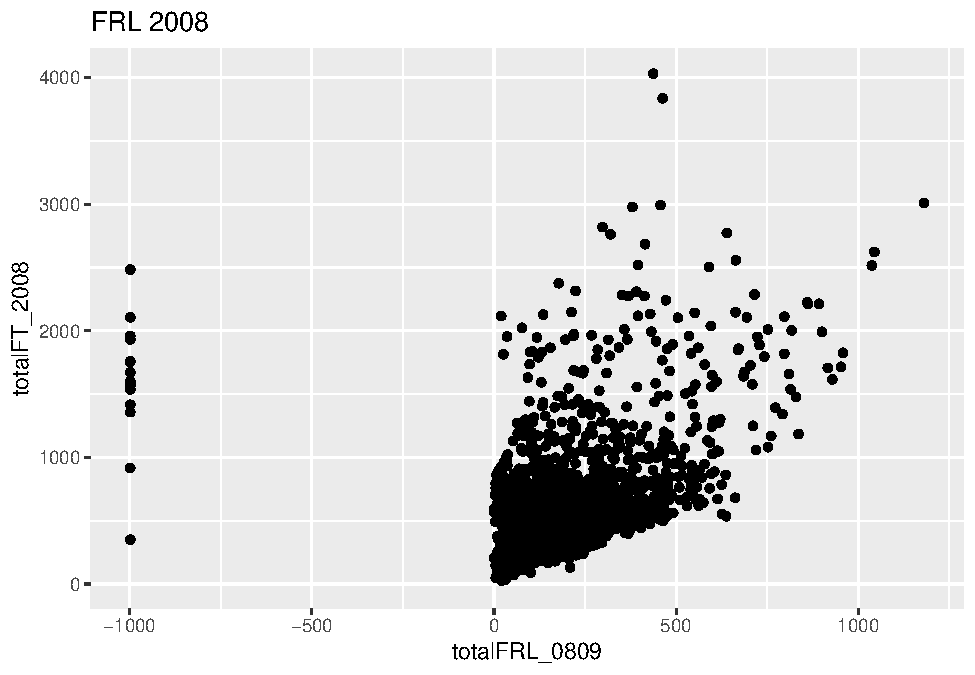
\includegraphics{test_course_notes_files/figure-latex/unnamed-chunk-37-1.pdf}

Let's see if we can fix it

\begin{Shaded}
\begin{Highlighting}[]
\NormalTok{newdf }\OperatorTok{\%\textgreater{}\%}\StringTok{ }
\StringTok{  }\KeywordTok{filter}\NormalTok{(}\OperatorTok{!}\KeywordTok{is.na}\NormalTok{(totalFRL\_}\DecValTok{0809}\NormalTok{)) }\OperatorTok{\%\textgreater{}\%}
\StringTok{  }\KeywordTok{ggplot}\NormalTok{(}\KeywordTok{aes}\NormalTok{(totalFRL\_}\DecValTok{0809}\NormalTok{, totalFT\_}\DecValTok{2008}\NormalTok{)) }\OperatorTok{+}
\StringTok{  }\KeywordTok{geom\_point}\NormalTok{() }\OperatorTok{+}
\StringTok{  }\KeywordTok{labs}\NormalTok{(}\DataTypeTok{title =} \StringTok{"FRL 2008"}\NormalTok{, }
       \DataTypeTok{x =} \StringTok{"totalFRL\_0809"}\NormalTok{) }\OperatorTok{+}
\StringTok{  }\KeywordTok{xlim}\NormalTok{(}\DecValTok{0}\NormalTok{, }\DecValTok{1000}\NormalTok{) }\OperatorTok{+}
\StringTok{  }\KeywordTok{ylim}\NormalTok{(}\DecValTok{0}\NormalTok{, }\DecValTok{1000}\NormalTok{)}
\end{Highlighting}
\end{Shaded}

\begin{verbatim}
## Warning: Removed 324 rows containing missing values (geom_point).
\end{verbatim}

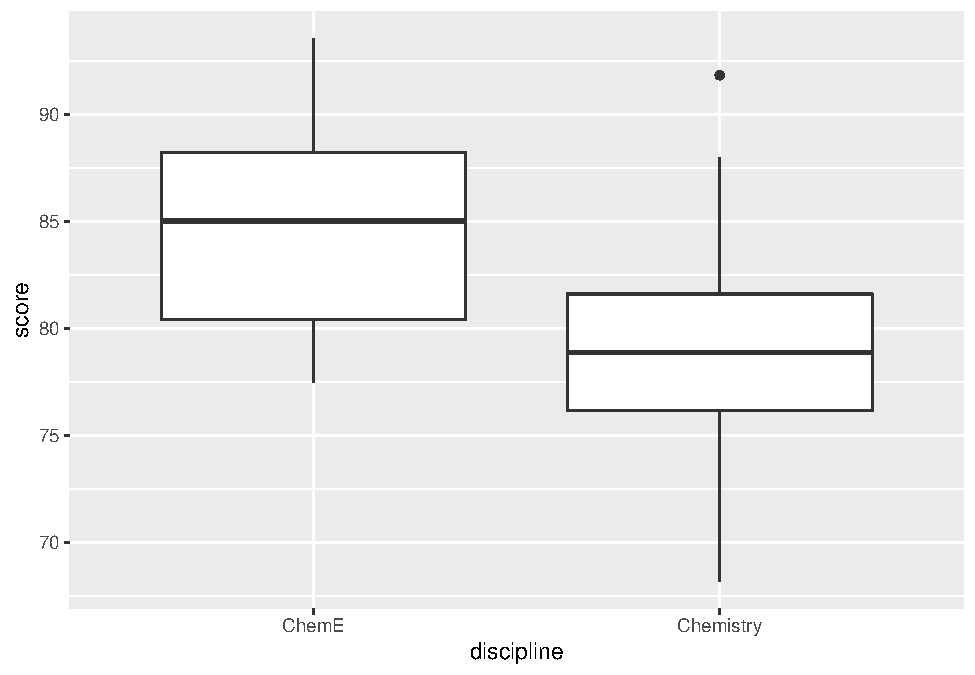
\includegraphics{test_course_notes_files/figure-latex/unnamed-chunk-38-1.pdf}

\hypertarget{applications}{%
\chapter{Applications}\label{applications}}

Some \emph{significant} applications are demonstrated in this chapter.

\hypertarget{example-one}{%
\section{Example one}\label{example-one}}

\hypertarget{example-two}{%
\section{Example two}\label{example-two}}

\hypertarget{final-words}{%
\chapter{Final Words}\label{final-words}}

We have finished a nice book.

  \bibliography{book.bib,packages.bib}

\end{document}
